% Created 2025-04-21 Mon 19:46
% Intended LaTeX compiler: pdflatex
\documentclass[12pt]{article}

%%%% settings when exporting code %%%% 

\usepackage{listings}
\lstdefinestyle{code-small}{
backgroundcolor=\color{white}, % background color for the code block
basicstyle=\ttfamily\small, % font used to display the code
commentstyle=\color[rgb]{0.5,0,0.5}, % color used to display comments in the code
keywordstyle=\color{black}, % color used to highlight certain words in the code
numberstyle=\ttfamily\tiny\color{gray}, % color used to display the line numbers
rulecolor=\color{black}, % color of the frame
stringstyle=\color[rgb]{0,.5,0},  % color used to display strings in the code
breakatwhitespace=false, % sets if automatic breaks should only happen at whitespace
breaklines=true, % sets automatic line breaking
columns=fullflexible,
frame=single, % adds a frame around the code (non,leftline,topline,bottomline,lines,single,shadowbox)
keepspaces=true, % % keeps spaces in text, useful for keeping indentation of code
literate={~}{$\sim$}{1}, % symbol properly display via latex
numbers=none, % where to put the line-numbers; possible values are (none, left, right)
numbersep=10pt, % how far the line-numbers are from the code
showspaces=false,
showstringspaces=false,
stepnumber=1, % the step between two line-numbers. If it's 1, each line will be numbered
tabsize=1,
xleftmargin=0cm,
emph={anova,apply,class,coef,colnames,colNames,colSums,dim,dcast,for,ggplot,head,if,ifelse,is.na,lapply,list.files,library,logLik,melt,plot,require,rowSums,sapply,setcolorder,setkey,str,summary,tapply},
aboveskip = \medskipamount, % define the space above displayed listings.
belowskip = \medskipamount, % define the space above displayed listings.
lineskip = 0pt} % specifies additional space between lines in listings
\lstset{style=code-small}
%%%% packages %%%%%

\usepackage[utf8]{inputenc}
\usepackage[T1]{fontenc}
\usepackage{lmodern}
\usepackage{textcomp}
\usepackage{color}
\usepackage{graphicx}
\usepackage{grffile}
\usepackage{wrapfig}
\usepackage{rotating}
\usepackage{longtable}
\usepackage{multirow}
\usepackage{multicol}
\usepackage{changes}
\usepackage{pdflscape}
\usepackage{geometry}
\usepackage[normalem]{ulem}
\usepackage{amssymb}
\usepackage{amsmath}
\usepackage{amsfonts}
\usepackage{dsfont}
\usepackage{array}
\usepackage{ifthen}
\usepackage{hyperref}
\usepackage{natbib}
\RequirePackage{setspace} % to modify the space between lines - incompatible with footnote in beamer
\renewcommand{\baselinestretch}{1.1}
\geometry{a4paper, left=10mm, right=10mm, top=10mm}
\usepackage{titlesec}
\usepackage{etoolbox}

\makeatletter
\patchcmd{\ttlh@hang}{\parindent\z@}{\parindent\z@\leavevmode}{}{}
\patchcmd{\ttlh@hang}{\noindent}{}{}{}
\makeatother
\RequirePackage{colortbl} % arrayrulecolor to mix colors
\definecolor{myorange}{rgb}{1,0.2,0}
\definecolor{mypurple}{rgb}{0.7,0,8}
\definecolor{mycyan}{rgb}{0,0.6,0.6}
\newcommand{\lightblue}{blue!50!white}
\newcommand{\darkblue}{blue!80!black}
\newcommand{\darkgreen}{green!50!black}
\newcommand{\darkred}{red!50!black}
\definecolor{gray}{gray}{0.5}
\hypersetup{
citecolor=[rgb]{0,0.5,0},
urlcolor=[rgb]{0,0,0.5},
linkcolor=[rgb]{0,0,0.5},
}
\newenvironment{note}{\small \color{gray}\fontfamily{lmtt}\selectfont}{\par}
\newenvironment{activity}{\color{orange}\fontfamily{qzc}\selectfont}{\par}
\RequirePackage{pifont}
\RequirePackage{relsize}
\newcommand{\Cross}{{\raisebox{-0.5ex}%
{\relsize{1.5}\ding{56}}}\hspace{1pt} }
\newcommand{\Valid}{{\raisebox{-0.5ex}%
{\relsize{1.5}\ding{52}}}\hspace{1pt} }
\newcommand{\CrossR}{ \textcolor{red}{\Cross} }
\newcommand{\ValidV}{ \textcolor{green}{\Valid} }
\usepackage{stackengine}
\usepackage{scalerel}
\newcommand\Warning[1][3ex]{%
\renewcommand\stacktype{L}%
\scaleto{\stackon[1.3pt]{\color{red}$\triangle$}{\tiny\bfseries !}}{#1}%
\xspace
}
\newcommand\Rlogo{\textbf{\textsf{R}}\xspace} %
\RequirePackage{fancyvrb}
\DefineVerbatimEnvironment{verbatim}{Verbatim}{fontsize=\small,formatcom = {\color[rgb]{0.5,0,0}}}
\RequirePackage{enumitem} % better than enumerate
\RequirePackage{epstopdf} % to be able to convert .eps to .pdf image files
\RequirePackage{capt-of} %
\RequirePackage{caption} % newlines in graphics
\RequirePackage{tikz-cd} % graph
\RequirePackage{booktabs} % for nice lines in table (e.g. toprule, bottomrule, midrule, cmidrule)
\RequirePackage{amsmath}
\RequirePackage{algorithm}
\RequirePackage[noend]{algpseudocode}
\RequirePackage{dsfont}
\RequirePackage{amsmath,stmaryrd,graphicx}
\RequirePackage{prodint} % product integral symbol (\PRODI)
\usepackage{ifthen}
\usepackage{xifthen}
\usepackage{xargs}
\usepackage{xspace}
\newcommand\defOperator[7]{%
\ifthenelse{\isempty{#2}}{
\ifthenelse{\isempty{#1}}{#7{#3}#4}{#7{#3}#4 \left#5 #1 \right#6}
}{
\ifthenelse{\isempty{#1}}{#7{#3}#4_{#2}}{#7{#3}#4_{#1}\left#5 #2 \right#6}
}
}
\newcommand\defUOperator[5]{%
\ifthenelse{\isempty{#1}}{
#5\left#3 #2 \right#4
}{
\ifthenelse{\isempty{#2}}{\underset{#1}{\operatornamewithlimits{#5}}}{
\underset{#1}{\operatornamewithlimits{#5}}\left#3 #2 \right#4}
}
}
\newcommand{\defBoldVar}[2]{
\ifthenelse{\equal{#2}{T}}{\boldsymbol{#1}}{\mathbf{#1}}
}
\newcommandx\Esp[2][1=,2=]{\defOperator{#1}{#2}{E}{}{\lbrack}{\rbrack}{\mathbb}}
\newcommandx\Prob[2][1=,2=]{\defOperator{#1}{#2}{P}{}{\lbrack}{\rbrack}{\mathbb}}
\newcommandx\Qrob[2][1=,2=]{\defOperator{#1}{#2}{Q}{}{\lbrack}{\rbrack}{\mathbb}}
\newcommandx\Var[2][1=,2=]{\defOperator{#1}{#2}{V}{ar}{\lbrack}{\rbrack}{\mathbb}}
\newcommandx\Cov[2][1=,2=]{\defOperator{#1}{#2}{C}{ov}{\lbrack}{\rbrack}{\mathbb}}
\newcommandx\Binom[2][1=,2=]{\defOperator{#1}{#2}{B}{}{(}{)}{\mathcal}}
\newcommandx\Gaus[2][1=,2=]{\defOperator{#1}{#2}{N}{}{(}{)}{\mathcal}}
\newcommandx\Wishart[2][1=,2=]{\defOperator{#1}{#2}{W}{ishart}{(}{)}{\mathcal}}
\newcommandx\Likelihood[2][1=,2=]{\defOperator{#1}{#2}{L}{}{(}{)}{\mathcal}}
\newcommandx\logLikelihood[2][1=,2=]{\defOperator{#1}{#2}{\ell}{}{(}{)}{}}
\newcommandx\Information[2][1=,2=]{\defOperator{#1}{#2}{I}{}{(}{)}{\mathcal}}
\newcommandx\Score[2][1=,2=]{\defOperator{#1}{#2}{S}{}{(}{)}{\mathcal}}
\newcommandx\Vois[2][1=,2=]{\defOperator{#1}{#2}{V}{}{(}{)}{\mathcal}}
\newcommandx\IF[2][1=,2=]{\defOperator{#1}{#2}{IF}{}{(}{)}{\mathcal}}
\newcommandx\Ind[1][1=]{\defOperator{}{#1}{1}{}{(}{)}{\mathds}}
\newcommandx\Max[2][1=,2=]{\defUOperator{#1}{#2}{(}{)}{min}}
\newcommandx\Min[2][1=,2=]{\defUOperator{#1}{#2}{(}{)}{max}}
\newcommandx\argMax[2][1=,2=]{\defUOperator{#1}{#2}{(}{)}{argmax}}
\newcommandx\argMin[2][1=,2=]{\defUOperator{#1}{#2}{(}{)}{argmin}}
\newcommandx\cvD[2][1=D,2=n \rightarrow \infty]{\xrightarrow[#2]{#1}}
\newcommandx\Hypothesis[2][1=,2=]{
\ifthenelse{\isempty{#1}}{
\mathcal{H}
}{
\ifthenelse{\isempty{#2}}{
\mathcal{H}_{#1}
}{
\mathcal{H}^{(#2)}_{#1}
}
}
}
\newcommandx\dpartial[4][1=,2=,3=,4=\partial]{
\ifthenelse{\isempty{#3}}{
\frac{#4 #1}{#4 #2}
}{
\left.\frac{#4 #1}{#4 #2}\right\rvert_{#3}
}
}
\newcommandx\dTpartial[3][1=,2=,3=]{\dpartial[#1][#2][#3][d]}
\newcommandx\ddpartial[3][1=,2=,3=]{
\ifthenelse{\isempty{#3}}{
\frac{\partial^{2} #1}{\partial #2^2}
}{
\frac{\partial^2 #1}{\partial #2\partial #3}
}
}
\newcommand\Real{\mathbb{R}}
\newcommand\Rational{\mathbb{Q}}
\newcommand\Natural{\mathbb{N}}
\newcommand\trans[1]{{#1}^\intercal}%\newcommand\trans[1]{{\vphantom{#1}}^\top{#1}}
\newcommand{\independent}{\mathrel{\text{\scalebox{1.5}{$\perp\mkern-10mu\perp$}}}}
\newcommand\half{\frac{1}{2}}
\newcommand\normMax[1]{\left|\left|#1\right|\right|_{max}}
\newcommand\normTwo[1]{\left|\left|#1\right|\right|_{2}}
\newcommand\Veta{\boldsymbol{\eta}}
\newcommand\VX{\mathbf{X}}
\author{Brice Ozenne}
\date{\today}
\title{Overview of the package BuyseTest}
\hypersetup{
 colorlinks=true,
 pdfauthor={Brice Ozenne},
 pdftitle={Overview of the package BuyseTest},
 pdfkeywords={},
 pdfsubject={},
 pdfcreator={Emacs 27.1 (Org mode 9.4.6)},
 pdflang={English}
 }
\begin{document}

\maketitle
This vignette describes the main functionalities of the \textbf{BuyseTest}
package, focusing on software (and not statistical) aspects, and assume
that the reader is familar with the GPC framework \footnote{if not,
\cite{buyse2010generalized} is a good place to start.}.

\bigskip

The BuyseTest package implements the Generalized Pairwise Comparisons
(GPC) as defined in \cite{buyse2010generalized} for complete
observations, and extended in \cite{peron2018extension} to deal with
right-censoring and \cite{piffoux2024restricted} to incorporate a
restriction time. When considering a single endpoint, the GPC
procedure can be summarized as follow. Denote the endpoint by \(Y\) in
the treatment group and by \(X\) in the control group. Given a
threshold of clinical relevance \(\tau\), the aim of GPC is to
estimate the proportion in favor of treatment\footnote{in absence of ties
this equals the Wilcoxon-Mann-Whitney parameter} \(\Prob[Y \geq X +
\tau]\) and the proportion in favor of control \(\Prob[X \geq Y +
\tau]\). Their difference \(\Prob[Y \geq X + \tau]-\Prob[X \geq Y +
\tau]\) leads to the net treatment benefit and their ratio
\(\frac{\Prob[Y \geq X + \tau]}{\Prob[X \geq Y + \tau]}\) to the win
ratio. The software also evaluate the proportion of neutral pairs
\(\Prob[ |X - Y| < \tau]\) and which can be included to obtain the
probabilistic index \(\Prob[Y \geq X + \tau] + 0.5 \Prob[ |X - Y| <
\tau]\) or win odds \(\frac{\Prob[Y \geq X + \tau] + 0.5 \Prob[ |X -
Y| < \tau] }{\Prob[X \geq Y + \tau] + 0.5\Prob[ |X - Y| < \tau]}\).
\begin{itemize}
\item the function \texttt{BuyseTest} performs the GPC procedure and is the main
function of the package. The user can interact with its output via
various methods:
\begin{itemize}
\item \texttt{summary} to obtain an overview of the results, including the
estimated net treatment benefit. The result table at the end of
the output can be directly access using \texttt{model.tables}.
\item \texttt{coef} to extract the estimates.
\item \texttt{confint} or \texttt{model.tables} to extract estimates, confidence intervals, and p.values.
\item \texttt{plot} for a graphical display of the scoring of the pair per endpoint.
\item \texttt{sensitivity} to perform a sensitivity analysis on the choice of the threshold(s).
\item \texttt{nobs} to extract the number of observations and pairs.
\item \texttt{getIid} to extract the iid decomposition of the estimator.
\item \texttt{getPairScore} to extract the contribution of each pair to the net treatment benefit.
\item \texttt{getSurvival} to extract the estimates of the survival used for right-censored endpoints.
\item \texttt{BuyseMultComp} to adjust p-values and confidence intervals for multiple comparisons.
\end{itemize}
\item the \texttt{powerBuyseTest} function performs simulation studies, e.g. to
estimate the statistical power or assess the bias / type 1 error
rate of a test for a specific design. The \texttt{simBuyseTest} function
can facilitate the definition of the data generating mechanism.
\item the \texttt{BuyseTest.options} function enables the user to access the
default values used in the \textbf{BuyseTest} package. The function can
also change the default values to better match the user needs.
\end{itemize}

Another vignette, "Wilcoxon test via GPC", details connexions between
GPC and the Wilcoxon rank sum test. Before going further we need to
load the \textbf{BuyseTest} package in the R session:
\lstset{language=r,label= ,caption= ,captionpos=b,numbers=none}
\begin{lstlisting}
library(BuyseTest)
library(data.table)
\end{lstlisting}

To illustrate the functionalities of the package, we will used the
\texttt{veteran} dataset from the \textbf{survival} package:
\lstset{language=r,label= ,caption= ,captionpos=b,numbers=none}
\begin{lstlisting}
data(cancer, package = "survival")
veteran <- cbind(id = 1:NROW(veteran), veteran)
veteran$trt <- factor(veteran$trt,1:2,c("Pl","Exp"))
head(veteran)
\end{lstlisting}

\begin{verbatim}
  id trt celltype time status karno diagtime age prior
1  1  Pl squamous   72      1    60        7  69     0
2  2  Pl squamous  411      1    70        5  64    10
3  3  Pl squamous  228      1    60        3  38     0
4  4  Pl squamous  126      1    60        9  63    10
5  5  Pl squamous  118      1    70       11  65    10
6  6  Pl squamous   10      1    20        5  49     0
\end{verbatim}


See \texttt{?veteran} for a presentation of the database.

\bigskip

\uline{Note:} the \textbf{BuyseTest} package is under active development. Newer
package versions may include additional functionalities and fix
previous bugs. The version of the package that is being is:
\lstset{language=r,label= ,caption= ,captionpos=b,numbers=none}
\begin{lstlisting}
utils::packageVersion("BuyseTest")
\end{lstlisting}

\begin{verbatim}
[1] ‘3.2.0’
\end{verbatim}


For completness, the details of the R session used to generate this
document are:
\lstset{language=r,label= ,caption= ,captionpos=b,numbers=none}
\begin{lstlisting}
sessionInfo()
\end{lstlisting}

\begin{verbatim}
R version 4.3.3 (2024-02-29)
Platform: x86_64-pc-linux-gnu (64-bit)
Running under: Ubuntu 22.04.5 LTS

Matrix products: default
BLAS:   /usr/lib/x86_64-linux-gnu/blas/libblas.so.3.10.0 
LAPACK: /usr/lib/x86_64-linux-gnu/lapack/liblapack.so.3.10.0

locale:
 [1] LC_CTYPE=en_US.UTF-8       LC_NUMERIC=C               LC_TIME=en_US.UTF-8       
 [4] LC_COLLATE=en_US.UTF-8     LC_MONETARY=en_US.UTF-8    LC_MESSAGES=en_US.UTF-8   
 [7] LC_PAPER=en_US.UTF-8       LC_NAME=C                  LC_ADDRESS=C              
[10] LC_TELEPHONE=C             LC_MEASUREMENT=en_US.UTF-8 LC_IDENTIFICATION=C       

time zone: Europe/Copenhagen
tzcode source: system (glibc)

attached base packages:
[1] stats     graphics  grDevices utils     datasets  methods   base     

other attached packages:
[1] data.table_1.16.2  BuyseTest_3.2.0    Rcpp_1.0.13        prodlim_2024.06.25
[5] ggplot2_3.5.1      survival_3.5-8    

loaded via a namespace (and not attached):
 [1] Matrix_1.6-5        gtable_0.3.5        future.apply_1.11.2 dplyr_1.1.4        
 [5] compiler_4.3.3      tidyselect_1.2.1    MatrixModels_0.5-3  parallel_4.3.3     
 [9] globals_0.16.3      splines_4.3.3       scales_1.3.0        lattice_0.22-5     
[13] R6_2.5.1            generics_0.1.3      future_1.34.0       tibble_3.2.1       
[17] munsell_0.5.1       pillar_1.9.0        rlang_1.1.4         utf8_1.2.4         
[21] cli_3.6.3           withr_3.0.1         magrittr_2.0.3      digest_0.6.37      
[25] grid_4.3.3          lifecycle_1.0.4     lava_1.8.0          vctrs_0.6.5        
[29] SparseM_1.81        glue_1.8.0          listenv_0.9.1       codetools_0.2-19   
[33] stats4_4.3.3        parallelly_1.38.0   fansi_1.0.6         colorspace_2.1-1   
[37] tools_4.3.3         pkgconfig_2.0.3
\end{verbatim}

\clearpage

\section{Performing generalized pairwise comparisons (GPC)}
\label{sec:org6fe3710}

To perform generalized pairwise comparisons, the \texttt{BuyseTest} function needs:
\begin{itemize}
\item where the data are stored \hfill \textcolor{orange}{- argument \texttt{data}}
\item the name of the endpoints \hfill \textcolor{orange}{- argument \texttt{endpoint}}
\item the type of each endpoint \hfill \textcolor{orange}{- argument \texttt{type}}
\item the variable defining the two treatment groups \hfill
\textcolor{orange}{- argument \texttt{treatment}}
\end{itemize}
The \texttt{BuyseTest} function has many optional arguments. For example:
\begin{itemize}
\item the threshold of clinical relevance associated to each endpoint \hfill \textcolor{orange}{- argument \texttt{threshold}}
\item the censoring associated to each endpoint (for time to event endpoints) \hfill \textcolor{orange}{- argument \texttt{status}}
\end{itemize}

\bigskip

There are two equivalent ways to define the GPC: 
\begin{itemize}
\item using a separate argument for each element:
\end{itemize}

\lstset{language=r,label= ,caption= ,captionpos=b,numbers=none}
\begin{lstlisting}
BT <- BuyseTest(data = veteran, 
                endpoint = "time", 
                type = "timeToEvent", 
                treatment = "trt", 
                status = "status", 
                threshold = 20)
\end{lstlisting}

\begin{verbatim}

         Generalized Pairwise Comparisons

Settings 
   - 2 groups  : Control = Pl and Treatment = Exp
   - 1 endpoint: 
       priority endpoint type           operator             threshold event       
       1        time     time to event  higher is favorable  20        status (0 1)
   - right-censored pairs: probabilistic score based on the survival curves 

Point estimation and calculation of the iid decomposition

Estimation of the estimator's distribution 
   - method: moments of the U-statistic

Gather the results in a S4BuyseTest object
\end{verbatim}

\clearpage

\begin{itemize}
\item or via a formula interface. In the formula interface endpoint are
wrapped by parentheses. The parentheses must be preceded by their
type: 
\begin{itemize}[label={-}]
\item binary (\texttt{b}, \texttt{bin}, or \texttt{binary})
\item continuous (\texttt{c}, \texttt{cont}, or  \texttt{continuous})
\item time to event (\texttt{t}, \texttt{tte}, or \texttt{timetoevent})
\end{itemize}
\end{itemize}
Here we also set the argument \texttt{trace} to \texttt{FALSE} to execute silently
the function:
\lstset{language=r,label= ,caption= ,captionpos=b,numbers=none}
\begin{lstlisting}
BT.f <- BuyseTest(trt ~ tte(time, threshold = 20, status = "status"),
                  data = veteran, trace = FALSE)
\end{lstlisting}

We can check that the two approaches are equivalent:
\lstset{language=r,label= ,caption= ,captionpos=b,numbers=none}
\begin{lstlisting}
BT.f@call <- list(); BT@call <- list();
testthat::expect_equal(BT.f,BT)
\end{lstlisting}

\subsection{Displaying the results}
\label{sec:org8ff92ea}

The results of the GPC can be displayed using the \texttt{summary} method:
\lstset{language=r,label= ,caption= ,captionpos=b,numbers=none}
\begin{lstlisting}
summary(BT)
\end{lstlisting}

\begin{verbatim}
       Generalized pairwise comparisons with 1 endpoint

 - statistic       : net treatment benefit  (delta: endpoint specific, Delta: global) 
 - null hypothesis : Delta == 0 
 - confidence level: 0.95 
 - inference       : H-projection of order 1 after atanh transformation 
 - treatment groups: Exp (treatment) vs. Pl (control) 
 - censored pairs  : probabilistic score based on the survival curves
 - results
 endpoint threshold total(%) favorable(%) unfavorable(%) neutral(%) uninf(%)   Delta
     time        20      100        37.78          46.54      15.68        0 -0.0877
 CI [2.5% ; 97.5%] p.value 
  [-0.2735;0.1045] 0.37162
\end{verbatim}


It displays information about each endpoint, percentage of pairs
classified as favorable, unfavorable, neutral, and uninformative, as
well as the estimated net treatment benefit (column \texttt{Delta}), its confidence
interval, and the corresponding p-value testing the absence of a group
difference. Other To display the number of pairs instead of the
percentage of pairs that are
favorable/unfavorable/neutral/uniformative, set the argument
\texttt{percentage} to \texttt{FALSE}. See \texttt{help(S4BuyseTest-summary)} for more
details about the \texttt{summary} method, its input and output. For a more
concise display of the results, consider using the \texttt{print} method:
\lstset{language=r,label= ,caption= ,captionpos=b,numbers=none}
\begin{lstlisting}
print(BT, percentage = FALSE)
\end{lstlisting}

\begin{verbatim}
endpoint threshold total favorable unfavorable neutral uninf   Delta CI [2.5% ; 97.5%]
    time        20  4692   1772.59     2183.89  735.52     0 -0.0877  [-0.2735;0.1045]
p.value
0.37162
\end{verbatim}


\bigskip

To access these values, we recommand using the \texttt{model.tables} method
that outputs the information from the previous table in a \texttt{data.frame}
format:

\lstset{language=r,label= ,caption= ,captionpos=b,numbers=none}
\begin{lstlisting}
model.tables(BT, percentage = FALSE)
\end{lstlisting}

\begin{verbatim}
  endpoint threshold total favorable unfavorable  neutral uninf       Delta   lower.ci
1     time        20  4692  1772.593    2183.886 735.5205     0 -0.08765836 -0.2735301
   upper.ci  p.value
1 0.1045245 0.371617
\end{verbatim}


\bigskip

An even more concise output can be obtained via the \texttt{confint} method:
\lstset{language=r,label= ,caption= ,captionpos=b,numbers=none}
\begin{lstlisting}
confint(BT)
\end{lstlisting}

\begin{verbatim}
            estimate         se   lower.ci  upper.ci null  p.value
time_t20 -0.08765836 0.09760901 -0.2735301 0.1045245    0 0.371617
\end{verbatim}


or \texttt{coef} method:
\lstset{language=r,label= ,caption= ,captionpos=b,numbers=none}
\begin{lstlisting}
coef(BT)
\end{lstlisting}

\begin{verbatim}
[1] -0.08765836
\end{verbatim}


\bigskip

\subsection{What about other summary statistics?}
\label{sec:org93f7185}

Results for other summary statistics are also accessible: \hfill \textcolor{orange}{- argument \texttt{statistic}}
\begin{itemize}
\item proportion in favor of treatment (\texttt{favorable}): \(\Prob[Y\geq X + \tau]\)
\item proportion in favor of control (\texttt{unfavorable}): \(\Prob[X\geq Y + \tau]\)
\item win ratio (\texttt{winRatio}): \(\frac{\Prob[Y\geq X + \tau]}{\Prob[X\geq Y + \tau]}\)
\end{itemize}

\noindent For instance, to display the estimated win ratio instead of
the estimated net treatment benefit, use:
\lstset{language=r,label= ,caption= ,captionpos=b,numbers=none}
\begin{lstlisting}
summary(BT, statistic = "winRatio")
\end{lstlisting}

\begin{verbatim}
       Generalized pairwise comparisons with 1 endpoint

 - statistic       : win ratio  (delta: endpoint specific, Delta: global) 
 - null hypothesis : Delta == 1 
 - confidence level: 0.95 
 - inference       : H-projection of order 1 after log transformation 
 - treatment groups: Exp (treatment) vs. Pl (control) 
 - censored pairs  : probabilistic score based on the survival curves
 - results
 endpoint threshold total(%) favorable(%) unfavorable(%) neutral(%) uninf(%)  Delta
     time        20      100        37.78          46.54      15.68        0 0.8117
 CI [2.5% ; 97.5%] p.value 
   [0.5134;1.2833] 0.37195
\end{verbatim}

\Warning In presence of ties, the null distribution of the proportion
in favor of treatment or control depends on the data generative
mechanism and the threshold of clinical relevance. This is why the
\texttt{confint} method will not produce any \texttt{p.value}:
\lstset{language=r,label= ,caption= ,captionpos=b,numbers=none}
\begin{lstlisting}
confint(BT, statistic = "favorable")
\end{lstlisting}

\begin{verbatim}
          estimate         se  lower.ci upper.ci null p.value
time_t20 0.3777905 0.04902199 0.2874747 0.477467   NA      NA
\end{verbatim}


unless the argument \texttt{null} is provided by the user. A permutation test
may be used to empirically estimate a value for the null hypothesis:
\lstset{language=r,label= ,caption= ,captionpos=b,numbers=none}
\begin{lstlisting}
BT.perm <- BuyseTest(trt ~ tte(time, threshold = 20, status = "status"),
                     data = veteran, trace = FALSE,
                     method.inference = "permutation", seed = 10)
confint(BT.perm, statistic = "favorable")
\end{lstlisting}

\begin{verbatim}
          estimate         se lower.ci upper.ci      null   p.value
time_t20 0.3777905 0.04770182       NA       NA 0.4205855 0.3636364
\end{verbatim}


which, in this example, is around 0.42. It worth noting that testing
an inadequate null hypothesis can have dramatic consequences on the
p-value:
\lstset{language=r,label= ,caption= ,captionpos=b,numbers=none}
\begin{lstlisting}
rbind(confint(BT, statistic = "favorable", null = 0.42),
      confint(BT, statistic = "favorable", null = 0.5))
\end{lstlisting}

\begin{verbatim}
           estimate         se  lower.ci upper.ci null    p.value
time_t20  0.3777905 0.04902199 0.2874747 0.477467 0.42 0.39826735
time_t201 0.3777905 0.04902199 0.2874747 0.477467 0.50 0.01673643
\end{verbatim}


\clearpage

\noindent Considering the proportion of neutral pairs in the summary
statistics: \hfill \textcolor{orange}{- argument \texttt{add.halfNeutral}}
\begin{itemize}
\item Wilcoxon-Mann-Whitney parameter or probabilistic index: \(\Prob[Y\geq X + \tau] + 0.5 \Prob[|Y- X| < \tau]\).
\item win odds: \(\frac{\Prob[Y\geq X + \tau] + 0.5 \Prob[|Y- X| < \tau]}{\Prob[X\geq Y + \tau] + 0.5 \Prob[|Y- X| < \tau]}\).
\end{itemize}
has been recommended (e.g. \cite{ajufo2023fallacies}) and these summary
statistics can be output by specifying the argument \texttt{add.halfNeutral}
to \texttt{TRUE} when calling \texttt{BuyseTest}:
\lstset{language=r,label= ,caption= ,captionpos=b,numbers=none}
\begin{lstlisting}
BT.half <- BuyseTest(trt ~ tte(time, threshold = 20, status = "status"),
                     data = veteran, trace = FALSE, add.halfNeutral = TRUE)
confint(BT.half, statistic = "favorable")
\end{lstlisting}

\begin{verbatim}
          estimate         se  lower.ci  upper.ci null   p.value
time_t20 0.4561708 0.04880921 0.3632263 0.5522714  0.5 0.3716632
\end{verbatim}


\lstset{language=r,label= ,caption= ,captionpos=b,numbers=none}
\begin{lstlisting}
confint(BT.half, statistic = "winRatio")
\end{lstlisting}

\begin{verbatim}
          estimate        se  lower.ci upper.ci null   p.value
time_t20 0.8388127 0.1650208 0.5704361 1.233454    1 0.3716211
\end{verbatim}


Testing a net treatment benefit of 0, a win odds of 1, or a
 Wilcoxon-Mann-Whitney parameter of 0.5 corresponds to the same
 hypothesis and therefore the same p-value should be obtained. The
 (small) discrepancy in p-values observed in this example (0.371617
 vs. 0.3716211 vs. 0.3716632) are due to small sample
 approximation. Such discrepancies will not arise when using
 non-parametric bootstrap or permutation tests using quantiles of the
 bootstrap or permutation distribution, e.g.:
\lstset{language=r,label= ,caption= ,captionpos=b,numbers=none}
\begin{lstlisting}
BT.halfperm <- BuyseTest(trt ~ tte(time, threshold = 20, status = "status"),
                         data = veteran, trace = FALSE, add.halfNeutral = TRUE,
                         method.inference = "bootstrap", seed = 10)
Mstat <- rbind(netBenefit = confint(BT.halfperm, statistic = "netBenefit"),
               winRatio = confint(BT.halfperm, statistic = "winRatio"),
               favorable = confint(BT.halfperm, statistic = "favorable"))
Mstat
\end{lstlisting}

\begin{verbatim}
              estimate         se   lower.ci  upper.ci null p.value
netBenefit -0.08765836 0.10021632 -0.2720510 0.1033974  0.0   0.383
winRatio    0.83881270 0.17440155  0.5722640 1.2306429  1.0   0.383
favorable   0.45617082 0.05010816  0.3639745 0.5516987  0.5   0.383
\end{verbatim}


\clearpage

\subsection{Stratified GPC}
\label{sec:orgce704d8}

GPC can be performed for subgroups of a categorical variable \hfill
\textcolor{orange}{- argument \texttt{strata}} \newline For
instance, the celltype may have huge influence on the survival time
and the investigator would like to only compare patients that have the
same celltype. In the formula interface this is achieved by adding a
single variable in the right hand side of the formula:
\lstset{language=r,label= ,caption= ,captionpos=b,numbers=none}
\begin{lstlisting}
ffstrata <- trt ~ tte(time, threshold = 20, status = "status") + celltype
BTstrata <- BuyseTest(ffstrata, data = veteran, trace = 0)
\end{lstlisting}

Not being wrapped by \texttt{bin}, \texttt{cont} or \texttt{tte} differentiates it from
endpoint variables. When doing a stratified analysis, the summary method
displays strata-specific and global results\footnote{the strata-specific
results can be removed by setting the argument \texttt{strata} to \texttt{"global"}
when calling \texttt{summary}.}:
\lstset{language=r,label= ,caption= ,captionpos=b,numbers=none}
\begin{lstlisting}
keep.colStrata <- c("endpoint","strata", "total",
                    "favorable","unfavorable","neutral","uninf","delta","Delta")
summary(BTstrata, type.display = keep.colStrata)
\end{lstlisting}

\begin{verbatim}
       Generalized pairwise comparisons with 1 endpoint and 4 strata

 - statistic       : net treatment benefit  (delta: endpoint specific, Delta: global) 
 - null hypothesis : Delta == 0 
 - confidence level: 0.95 
 - inference       : H-projection of order 1 after atanh transformation 
 - treatment groups: Exp (treatment) vs. Pl (control) 
 - strata weights  : 26.38%, 34.63%, 18.47%, 20.52% 
 - uninformative pairs: no contribution
 - results
 endpoint    strata total(%) favorable(%) unfavorable(%) neutral(%) uninf(%)   delta   Delta
     time    global   100.00        36.06          45.77      17.33     0.85 -0.0997 -0.0997
           squamous    25.38        14.33           8.77       2.28     0.00  0.2193        
          smallcell    45.69        12.69          20.88      11.27     0.85 -0.1792        
              adeno    13.71         4.74           6.15       2.81     0.00 -0.1034        
              large    15.23         4.30           9.97       0.96     0.00 -0.3722
\end{verbatim}


The percentage of pairs in the
total/favorable/unfavorable/neutral/uninf columns are relative to the
overall number of pairs whereas the column \texttt{delta} presents the
endpoint and strata-specific net treatment benefits (in the last 4
lines). The last column (\texttt{Delta}) displays the global (i.e. pooled
over strata), conditional, net treatment benefit. \newline \Warning
With this weighting scheme the proportion of favorable pairs minus the
proportion of unfavorable pairs (\texttt{36.06\%-45.77\%=9.71\%}) does not equal
the global net treatment benefit (\texttt{9.97\%}). To retrieve the net
treatment benefits, we first extract the number of pairs per strata
using the method \texttt{nobs}:
\lstset{language=r,label= ,caption= ,captionpos=b,numbers=none}
\begin{lstlisting}
strata.obs <- as.data.frame(nobs(BTstrata, strata = TRUE))
strata.obs
\end{lstlisting}

\begin{verbatim}
          Pl Exp pairs
squamous  15  20   300
smallcell 30  18   540
adeno      9  18   162
large     15  12   180
\end{verbatim}


and use the method \texttt{model.tables} to extract the number of favorable and unfavorable
pairs per strata:
\lstset{language=r,label= ,caption= ,captionpos=b,numbers=none}
\begin{lstlisting}
dfStrata <- model.tables(BTstrata, percentage = FALSE,
                         strata = c("squamous","smallcell","adeno","large"),
                         columns = c("strata","total","favorable","unfavorable"))
dfStrata
\end{lstlisting}

\begin{verbatim}
     strata total favorable unfavorable
2  squamous   300 169.40260    103.6104
3 smallcell   540 150.00000    246.7778
4     adeno   162  56.00000     72.7500
5     large   180  50.83333    117.8333
\end{verbatim}


We retrieve the strata-specific net treatment benefits by comparing, in each
strata, the number of favorable and unfavorable pairs relative to the
number of pairs\footnote{Alernatively one could compute, from the \texttt{summary}, the difference
between the percentage of favorable and unfavorable pairs relative to
the percentage of pairs in the strata, e.g. \((14.33\%-8.77\%)/25.38\%
\approx 21.93\%\)}:
\lstset{language=r,label= ,caption= ,captionpos=b,numbers=none}
\begin{lstlisting}
delta <- (dfStrata$favorable - dfStrata$unfavorable)/strata.obs$pairs
delta
\end{lstlisting}

\begin{verbatim}
[1]  0.2193074 -0.1792181 -0.1033951 -0.3722222
\end{verbatim}


The global net treatment benefit is then the sum of the strata-specific net
treatment benefits weighted by the strata weights:
\lstset{language=r,label= ,caption= ,captionpos=b,numbers=none}
\begin{lstlisting}
weightCMH <- strata.obs$pairs/(strata.obs$Pl + strata.obs$Exp)

list(estimate = sum(delta * weightCMH/sum(weightCMH)),
     weight = 100*weightCMH/sum(weightCMH))
\end{lstlisting}

\begin{verbatim}
$estimate
[1] -0.09967584

$weight
[1] 26.38329 34.62807 18.46830 20.52034
\end{verbatim}


\Warning One exception is for the win ratio and win odds where the
ratio between the global proportions is taken, i.e., pooling is
performed at the numerator and at the denominator instead of pooling
fractions - see \cite{dong2018stratified}, equation 1.


\clearpage

The default weighting scheme is \texttt{CMH}, standing for
Cochran-Mantel-Haenszel, which has been recommaned in the litterature
\citep{dong2018stratified}. It is efficient under the assumption of a
common multiplicative effect (across strata) on the odds ratio
scale. 

\bigskip 

Other weighting schemes can be used. \hfill \textcolor{orange}{-
argument \texttt{pool.strata}}. \newline For instance, if the effect is
thought additive, one should instead weight proportionnaly to the
number of pairs:
\lstset{language=r,label= ,caption= ,captionpos=b,numbers=none}
\begin{lstlisting}
BTstrata2 <- BuyseTest(ffstrata, data = veteran, trace = 0, pool.strata = "buyse")
summary(BTstrata2, type.display = keep.colStrata)
\end{lstlisting}

\begin{verbatim}
       Generalized pairwise comparisons with 1 endpoint and 4 strata

 - statistic       : net treatment benefit  (delta: endpoint specific, Delta: global) 
 - null hypothesis : Delta == 0 
 - confidence level: 0.95 
 - inference       : H-projection of order 1 after atanh transformation 
 - treatment groups: Exp (treatment) vs. Pl (control) 
 - strata weights  : 25.38%, 45.69%, 13.71%, 15.23% 
 - uninformative pairs: no contribution
 - results
 endpoint    strata total(%) favorable(%) unfavorable(%) neutral(%) uninf(%)   delta   Delta
     time    global   100.00        36.06          45.77      17.33     0.85 -0.0971 -0.0971
           squamous    25.38        14.33           8.77       2.28     0.00  0.2193        
          smallcell    45.69        12.69          20.88      11.27     0.85 -0.1792        
              adeno    13.71         4.74           6.15       2.81     0.00 -0.1034        
              large    15.23         4.30           9.97       0.96     0.00 -0.3722
\end{verbatim}

The weighting scheme only affect the evaluation of the overall net
treatment benefit, which now equals the difference between the overall
proportion of favorable vs. unfavorable pairs (\texttt{36.06\%-45.77\%}). While
extractors will by default output global estimates (i.e. after pooling
the results over strata)
\lstset{language=r,label= ,caption= ,captionpos=b,numbers=none}
\begin{lstlisting}
confint(BTstrata2)
\end{lstlisting}

\begin{verbatim}
            estimate        se   lower.ci   upper.ci null  p.value
time_t20 -0.09706901 0.0977929 -0.2829348 0.09582321    0 0.323961
\end{verbatim}


one can specify the argument \texttt{strata} to extract strata-specific estimates:
\lstset{language=r,label= ,caption= ,captionpos=b,numbers=none}
\begin{lstlisting}
confint(BTstrata, strata = TRUE)
\end{lstlisting}

\begin{verbatim}
                     estimate        se   lower.ci  upper.ci null   p.value
time_t20.squamous   0.2193074 0.1911515 -0.1690137 0.5486919    0 0.2669352
time_t20.smallcell -0.1792181 0.1540933 -0.4567640 0.1301230    0 0.2551275
time_t20.adeno     -0.1033951 0.2465197 -0.5314450 0.3667172    0 0.6771002
time_t20.large     -0.3722222 0.2190018 -0.7110335 0.1068610    0 0.1240457
\end{verbatim}


\Warning The previous weighting scheme leads to the estimatation of a
conditional net treatment benefit, which will generally differ from
the marginal (i.e. non-adjusted) net treatment benefit. To retrieve a
marginal effect while adjusting for covariate, one can use
standardization:
\lstset{language=r,label= ,caption= ,captionpos=b,numbers=none}
\begin{lstlisting}
BTstd <- BuyseTest(ffstrata, data = veteran, trace = 0, pool.strata = "standardization")
model.tables(BTstd)[,c("strata","total","delta","Delta","lower.ci","upper.ci","p.value")]
\end{lstlisting}

\begin{verbatim}
               strata      total       delta     Delta   lower.ci   upper.ci   p.value
1              global 100.000000 -0.11874500 -0.118745 -0.3037001 0.07483473 0.2287434
2            squamous   6.393862  0.21930736        NA         NA         NA        NA
3  smallcell.squamous  12.787724  0.35699653        NA         NA         NA        NA
4      adeno.squamous   3.836317  0.41018519        NA         NA         NA        NA
5      large.squamous   6.393862  0.03622106        NA         NA         NA        NA
6  squamous.smallcell   5.754476 -0.50654161        NA         NA         NA        NA
7           smallcell  11.508951 -0.17921811        NA         NA         NA        NA
8     adeno.smallcell   3.452685 -0.25308642        NA         NA         NA        NA
9     large.smallcell   5.754476 -0.80740741        NA         NA         NA        NA
10     squamous.adeno   5.754476 -0.41165224        NA         NA         NA        NA
11    smallcell.adeno  11.508951 -0.02906379        NA         NA         NA        NA
12              adeno   3.452685 -0.10339506        NA         NA         NA        NA
13        large.adeno   5.754476 -0.76311728        NA         NA         NA        NA
14     squamous.large   3.836317 -0.04494949        NA         NA         NA        NA
15    smallcell.large   7.672634  0.25946502        NA         NA         NA        NA
16        adeno.large   2.301790  0.21296296        NA         NA         NA        NA
17              large   3.836317 -0.37222222        NA         NA         NA        NA
\end{verbatim}

i.e. evaluate the net treatment benefit for every combination of
strate between the control and active group (either identical or
differen across the two groups) and pool the results. See chapter 9 of
\cite{buyse2025gpc} for further explanations.

\clearpage

\subsection{Using multiple endpoints}
\label{sec:org64d15e7}

More than one endpoint can be considered by indicating a vector of
endpoints, types, and thresholds. In the formula interface, the
different endpoints must be separated with a "+" on the right hand
side of the formula:
\lstset{language=r,label= ,caption= ,captionpos=b,numbers=none}
\begin{lstlisting}
ff2 <- trt ~ tte(time, threshold = 20, status = "status") + cont(karno, threshold = 0)
BT.H <- BuyseTest(ff2, data = veteran, trace = 0)
summary(BT.H)
\end{lstlisting}

\begin{verbatim}
       Generalized pairwise comparisons with 2 prioritized endpoints

 - statistic       : net treatment benefit  (delta: endpoint specific, Delta: global) 
 - null hypothesis : Delta == 0 
 - confidence level: 0.95 
 - inference       : H-projection of order 1 after atanh transformation 
 - treatment groups: Exp (treatment) vs. Pl (control) 
 - censored pairs  : probabilistic score based on the survival curves
 - neutral pairs   : re-analyzed using lower priority endpoints
 - results
 endpoint threshold total(%) favorable(%) unfavorable(%) neutral(%) uninf(%)   delta   Delta
     time        20   100.00        37.78          46.54      15.68        0 -0.0877 -0.0877
    karno              15.68         5.78           7.11       2.78        0 -0.0133 -0.1009
 CI [2.5% ; 97.5%] p.value 
  [-0.2735;0.1045] 0.37162 
  [-0.2901;0.0959] 0.31478
\end{verbatim}

The hierarchy of the endpoint is defined from left (most important
endpoint, here \texttt{time}) to right (least important endpoint, here
\texttt{karno}). In the \texttt{summary} output, the confidence intervals and
p.values are computed for the column \texttt{Delta}, i.e. here -8.77\% is the
net treatment benefit for the first endpoint (line 1) and -10.09\% is the net
treatment benefit for the first and second endpoint (line 2). In other words,
the last confidence interval and p-value is the one for the analysis
over all endpoints (generally the one to report).

\bigskip

A graphical representation of the GPC procedure can be obtained by the
\texttt{plot} method. It will display the percentage of favorable,
unfavorable, neutral, and uninformative pairs per endpoint. Three
(equivalent) graphical display are possible, the first one (\texttt{"hist"})
being the recommanded one:
\lstset{language=r,label= ,caption= ,captionpos=b,numbers=none}
\begin{lstlisting}
plot(BT.H, type = "hist")
plot(BT.H, type = "pie")
plot(BT.H, type = "racetrack")
\end{lstlisting}

\begin{center}
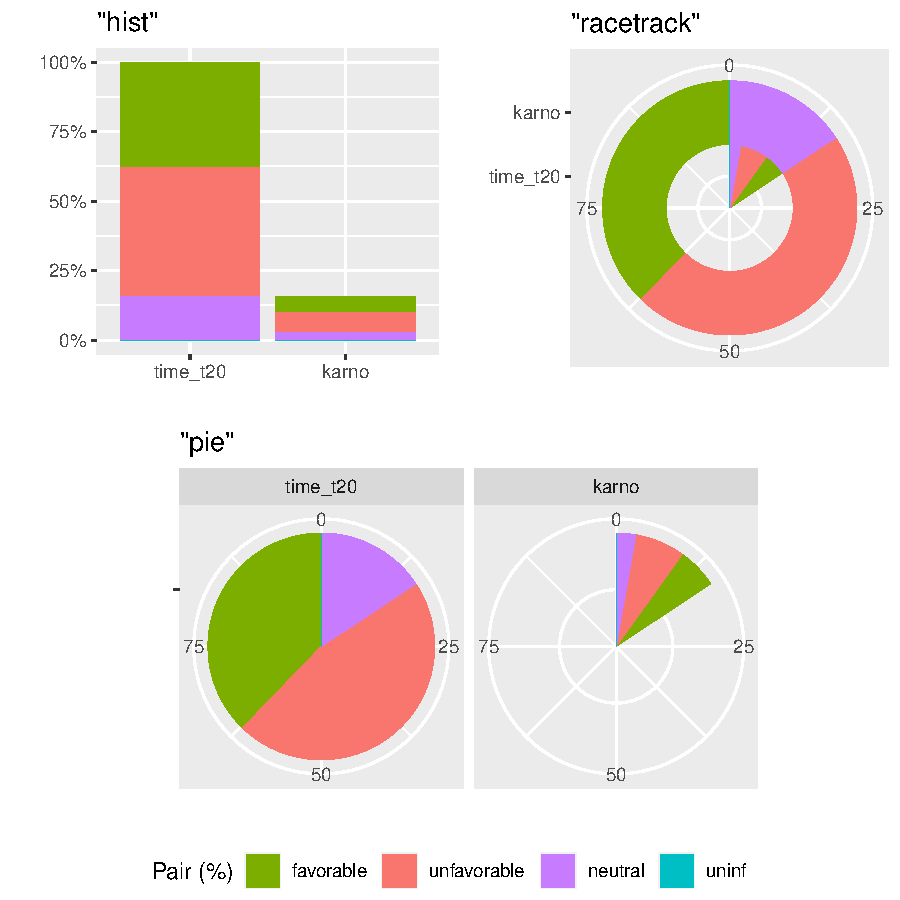
\includegraphics[trim={0 0 0 0},width=0.7\textwidth]{./figures/plot-BuyseTest.pdf}
\end{center}


\bigskip

It is also possible to perform the comparisons on all pairs for all
endpoints by setting the argument \texttt{hierarchical} to \texttt{FALSE}:
\lstset{language=r,label= ,caption= ,captionpos=b,numbers=none}
\begin{lstlisting}
BT.nH <- BuyseTest(ff2, hierarchical = FALSE, data = veteran, trace = 0)
summary(BT.nH)
\end{lstlisting}

\begin{verbatim}
       Generalized pairwise comparisons with 2 endpoints

 - statistic       : net treatment benefit  (delta: endpoint specific, Delta: global) 
 - null hypothesis : Delta == 0 
 - confidence level: 0.95 
 - inference       : H-projection of order 1 after atanh transformation 
 - treatment groups: Exp (treatment) vs. Pl (control) 
 - censored pairs  : probabilistic score based on the survival curves
 - results
 endpoint threshold weight total(%) favorable(%) unfavorable(%) neutral(%) uninf(%)   delta
     time        20    0.5      100        37.78          46.54      15.68        0 -0.0877
    karno              0.5      100        41.82          44.95      13.24        0 -0.0313
   Delta CI [2.5% ; 97.5%] p.value 
 -0.0438  [-0.1388;0.0519] 0.36977 
 -0.0595  [-0.2267;0.1111] 0.49514
\end{verbatim}

In that case the score of a pair is the weighted sum of the score
relative to each endpoint. By default, the weights are all set to the
same value but this behavior can be changed by setting the argument
\texttt{weight} when calling \texttt{BuyseTest}, e.g.:
\lstset{language=r,label= ,caption= ,captionpos=b,numbers=none}
\begin{lstlisting}
ff2w <- trt ~ tte(time, threshold = 20, status = "status", weight = 0.8)
ff2w <- update.formula(ff2w, . ~ . + cont(karno, threshold = 0, weight = 0.2))
BT.nHw <- BuyseTest(ff2w, hierarchical = FALSE, data = veteran, trace = 0)
model.tables(BT.nHw)
\end{lstlisting}

\begin{verbatim}
  endpoint threshold weight total favorable unfavorable  neutral uninf       delta
1     time     2e+01    0.8   100  37.77905    46.54489 15.67606     0 -0.08765836
3    karno     1e-12    0.2   100  41.81586    44.94885 13.23529     0 -0.03132992
        Delta   lower.ci   upper.ci   p.value
1 -0.07012668 -0.2203714 0.08336855 0.3707289
3 -0.07639267 -0.2503756 0.10237001 0.4026905
\end{verbatim}


This has been refered as the O’Brien test in the litterature
(\cite{verbeeck2019generalized}, section 3.2). Alternatively, one may be
interested in the endpoint specific results. This can be performed
by applying the \texttt{BuyseTest} function separately to each endpoint, e.g.:
\lstset{language=r,label= ,caption= ,captionpos=b,numbers=none}
\begin{lstlisting}
confint(BuyseTest(trt ~ cont(karno, threshold = 0), data = veteran, trace = 0))
\end{lstlisting}

\begin{verbatim}
         estimate         se   lower.ci  upper.ci null   p.value
karno -0.03132992 0.09787113 -0.2197111 0.1593037    0 0.7490407
\end{verbatim}


or setting the argument \texttt{cumulative} to \texttt{FALSE} when calling the
\texttt{confint} function:
\lstset{language=r,label= ,caption= ,captionpos=b,numbers=none}
\begin{lstlisting}
confint(BT.nHw, cumulative = FALSE)
\end{lstlisting}

\begin{verbatim}
            estimate         se   lower.ci  upper.ci null   p.value
time_t20 -0.08765836 0.09760901 -0.2735301 0.1045245    0 0.3716170
karno    -0.03132992 0.09787113 -0.2197111 0.1593037    0 0.7490407
\end{verbatim}


\bigskip

Note: the apparent discrepency in p-value between the hierarchical and
non-hierarchical GPC at the first priority (0.3762 vs 0.3698 vs
0-3707) is due to the use of a transformation that makes the p-value
dependent on the estimate. Otherwise the p-value would be the same at
the first priority, e.g.:
\lstset{language=r,label= ,caption= ,captionpos=b,numbers=none}
\begin{lstlisting}
confint(BT.nHw, transform = FALSE)
\end{lstlisting}

\begin{verbatim}
            estimate         se   lower.ci   upper.ci null   p.value
time_t20 -0.07012668 0.07808721 -0.2231748 0.08292143    0 0.3691557
karno    -0.07639267 0.09093303 -0.2546181 0.10183280    0 0.4008534
\end{verbatim}



\clearpage

\subsection{Statistical inference}
\label{sec:org9c2c2a6}

Uncertainty about the estimates can be quantified using: \hfill \textcolor{orange}{- argument \texttt{method.inference}}
\begin{itemize}
\item \textbf{permutation test} (\texttt{"permutation"}). Assuming exchangeability under the null hypothesis,
this approach gives valid p-values (regardless to the sample size)
for testing the absence of a difference between the groups.
\end{itemize}
\lstset{language=r,label= ,caption= ,captionpos=b,numbers=none}
\begin{lstlisting}
BT.perm <- BuyseTest(trt ~ tte(time, threshold = 20, status = "status"),
                     data = veteran, trace = 0, method.inference = "permutation",
                     seed = 10) 
summary(BT.perm)
\end{lstlisting}

\begin{verbatim}
       Generalized pairwise comparisons with 1 endpoint

 - statistic       : net treatment benefit  (delta: endpoint specific, Delta: global) 
 - null hypothesis : Delta == 0 
 - confidence level: 0.95 
 - inference       : permutation test with 1000 samples 
                     p-value computed using the permutation distribution 
 - treatment groups: Exp (treatment) vs. Pl (control) 
 - censored pairs  : probabilistic score based on the survival curves
 - results
 endpoint threshold total(%) favorable(%) unfavorable(%) neutral(%) uninf(%)   Delta p.value 
     time        20      100        37.78          46.54      15.68        0 -0.0877 0.35265
\end{verbatim}

\begin{itemize}
\item \textbf{bootstrap resampling} (\texttt{"bootstrap"}). In large enough samples, this approach gives valid
p-values and confidence intervals.
\end{itemize}

\lstset{language=r,label= ,caption= ,captionpos=b,numbers=none}
\begin{lstlisting}
BT.boot <- BuyseTest(trt ~ tte(time, threshold = 20, status = "status"),
                     data = veteran, trace = 0, method.inference = "bootstrap",
                     seed = 10) 
summary(BT.boot)
\end{lstlisting}

\begin{verbatim}
       Generalized pairwise comparisons with 1 endpoint

 - statistic       : net treatment benefit  (delta: endpoint specific, Delta: global) 
 - null hypothesis : Delta == 0 
 - confidence level: 0.95 
 - inference       : bootstrap resampling with 1000 samples 
                     CI computed using the percentile method; p-value by test inversion 
 - treatment groups: Exp (treatment) vs. Pl (control) 
 - censored pairs  : probabilistic score based on the survival curves
 - results
 endpoint threshold total(%) favorable(%) unfavorable(%) neutral(%) uninf(%)   Delta
     time        20      100        37.78          46.54      15.68        0 -0.0877
 CI [2.5% ; 97.5%] p.value 
  [-0.2721;0.1034]   0.383
\end{verbatim}

\begin{itemize}
\item \textbf{asymptotic distribution} (\texttt{"u-statistic"}). In large enough
samples, this approach gives valid p-values and confidence intervals
\citep{ozenne2021asymptotic}.
\end{itemize}

\lstset{language=r,label= ,caption= ,captionpos=b,numbers=none}
\begin{lstlisting}
BT.ustat <- BuyseTest(trt ~ tte(time, threshold = 20, status = "status"),
                      data = veteran, trace = 0, method.inference = "u-statistic") 
summary(BT.ustat)
\end{lstlisting}

\begin{verbatim}
       Generalized pairwise comparisons with 1 endpoint

 - statistic       : net treatment benefit  (delta: endpoint specific, Delta: global) 
 - null hypothesis : Delta == 0 
 - confidence level: 0.95 
 - inference       : H-projection of order 1 after atanh transformation 
 - treatment groups: Exp (treatment) vs. Pl (control) 
 - censored pairs  : probabilistic score based on the survival curves
 - results
 endpoint threshold total(%) favorable(%) unfavorable(%) neutral(%) uninf(%)   Delta
     time        20      100        37.78          46.54      15.68        0 -0.0877
 CI [2.5% ; 97.5%] p.value 
  [-0.2735;0.1045] 0.37162
\end{verbatim}

The first two approaches require simulating a large number of samples
and applying the GPC to each of these samples. The \texttt{seed} argument is
used to generate a seed for each sample. The number of samples is set
using the arugment \texttt{n.resampling} and it should large enough to limit
the Monte Carlo error when estimating the p-value. Typically should be
at least 10000 to get, roughtly, 2-digit precision, as examplified
below:
\lstset{language=r,label= ,caption= ,captionpos=b,numbers=none}
\begin{lstlisting}
set.seed(10)
sapply(1:10, function(i){mean(rbinom(1e4, size = 1, prob = 0.05))})
\end{lstlisting}

\begin{verbatim}
[1] 0.0511 0.0491 0.0489 0.0454 0.0516 0.0522 0.0468 0.0483 0.0491 0.0508
\end{verbatim}

Indeed, here we get a reasonnable approximation of \texttt{0.05} (if we round
and only keep 2 digits). Note that to get 3 digits precision we would
need more samples. The last method does not rely on resampling but on
the computation of the influence function of the
estimator. Fortunately, when using the Gehan's scoring rule, this does
not really involve any extra-calculations and this is therefore very
fast to perform. When using the Peron's scoring rule, more serious
extra-calculations are involved so the computation time is expected to
increase by a factor 5 to 10 compared to the point estimate alone
(i.e. \texttt{method.inference} equal to \texttt{"none"}).

\bigskip

It is possible to relax the exchangeability assumption using a
studentized permutation. A studentized bootstrap is also possible to
improve on the better small samples properties of the bootstrap
confidence intervals. Both rely on the asymptotic approach to estimate
standard errors and are more numerically intensive.

\clearpage

\subsection{What if smaller is better?}
\label{sec:org3f9794d}
By default \texttt{BuyseTest} will always assume that higher values of an
endpoint are favorable. This behavior can be changed by specifying \texttt{operator = "<0"}
for an endpoint:
\lstset{language=r,label= ,caption= ,captionpos=b,numbers=none}
\begin{lstlisting}
ffop <- trt ~ tte(time, status = "status", threshold = 20, operator = "<0")
BTinv <- BuyseTest(ffop, data = veteran, trace = 0)
summary(BTinv)
\end{lstlisting}

\begin{verbatim}
       Generalized pairwise comparisons with 1 endpoint

 - statistic       : net treatment benefit  (delta: endpoint specific, Delta: global) 
 - null hypothesis : Delta == 0 
 - confidence level: 0.95 
 - inference       : H-projection of order 1 after atanh transformation 
 - treatment groups: Exp (treatment) vs. Pl (control) 
 - censored pairs  : probabilistic score based on the survival curves
 - results
 endpoint threshold total(%) favorable(%) unfavorable(%) neutral(%) uninf(%)  Delta
     time        20      100        46.54          37.78      15.68        0 0.0877
 CI [2.5% ; 97.5%] p.value 
  [-0.1045;0.2735] 0.37162
\end{verbatim}

Internally \texttt{BuyseTest} will compute the favorable and unfavorable
score as usual and then switch them around if the operator equals
\texttt{"<0"}.

\clearpage

\subsection{Stopping comparison for neutral pairs}
\label{sec:org0dbc8af}
In presence of neutral pairs, \texttt{BuyseTest} will, by default, continue
the comparison on the endpoints with lower priority. For instance let
consider a dataset with one observation in each treatment arm:
\lstset{language=r,label= ,caption= ,captionpos=b,numbers=none}
\begin{lstlisting}
dt.sim <- data.table(Id = 1:2,
                     treatment = c("Yes","No"),
                     tumor = c("Yes","Yes"),
                     size = c(15,20))
dt.sim
\end{lstlisting}

\begin{verbatim}
      Id treatment  tumor  size
   <int>    <char> <char> <num>
1:     1       Yes    Yes    15
2:     2        No    Yes    20
\end{verbatim}


\bigskip

If we use the GPC with tumor as the first endpoint and size as the
second endpoint:
\lstset{language=r,label= ,caption= ,captionpos=b,numbers=none}
\begin{lstlisting}
BT.pair <- BuyseTest(treatment ~ bin(tumor) + cont(size, operator = "<0"), data = dt.sim,
                     trace = 0, method.inference = "none")
summary(BT.pair)
\end{lstlisting}

\begin{verbatim}
      Generalized pairwise comparisons with 2 prioritized endpoints

- statistic       : net treatment benefit  (delta: endpoint specific, Delta: global) 
- treatment groups: Yes (treatment) vs. No (control) 
- neutral pairs   : re-analyzed using lower priority endpoints
- results
endpoint total(%) favorable(%) unfavorable(%) neutral(%) uninf(%) delta Delta
   tumor      100            0              0        100        0     0     0
    size      100          100              0          0        0     1     1
\end{verbatim}


the outcome of the comparison is neutral for the first priority, but
favorable for the second. Setting the argument \texttt{neutral.as.uninf} to
\texttt{FALSE} will stop the comparison when a pair is classified as neutral:
\lstset{language=r,label= ,caption= ,captionpos=b,numbers=none}
\begin{lstlisting}
BT.pair2 <- BuyseTest(treatment ~ bin(tumor) + cont(size, operator = "<0"), data = dt.sim,
                     trace = 0, method.inference = "none", neutral.as.uninf = FALSE)
summary(BT.pair2)
\end{lstlisting}

\begin{verbatim}
      Generalized pairwise comparisons with 2 prioritized endpoints

- statistic       : net treatment benefit  (delta: endpoint specific, Delta: global) 
- treatment groups: Yes (treatment) vs. No (control) 
- neutral pairs   : ignored at lower priority endpoints
- results
endpoint total(%) favorable(%) unfavorable(%) neutral(%) uninf(%) delta Delta
   tumor      100            0              0        100        0     0     0
    size        0            0              0          0        0     0     0
\end{verbatim}


So in this case no pair is analyzed at second priority.

\clearpage


\subsection{Is multiple testing a concern with GPC?}
\label{sec:org3e0e444}

Yes, as with any other statistical method. Having a pre-defined
statistical plan (i.e. written before looking at the data) specifying
the hierarchy of endpoints, their threshold of clinical relevance is
recommanded. When planning multiple GPC, summarize the results can be
done via one of two principles:
\begin{itemize}
\item \textbf{intersection union principle}: one rejects the (global) null
hypothesis if there is evidence for an effect in all the GPC
analyses. This is typically a sensitivity analysis: checking that
the results are not too sensitive to the choice of an
hyperparameter. No multiplicity adjustment is needed other than
considering the largest p-value among all tests. For instance, when
checking whether the estimated net treatment benefit is similar across a range
of threshold of clincial relevance, we would obtain a p-value of
0.76
\end{itemize}
\lstset{language=r,label= ,caption= ,captionpos=b,numbers=none}
\begin{lstlisting}
BTse <- sensitivity(BT.ustat, threshold = seq(0,500, length.out=10),
                          trace = FALSE)
BTse
\end{lstlisting}

\begin{verbatim}
        time    estimate         se    lower.ci   upper.ci null   p.value
1    0.00000 -0.08752774 0.10041203 -0.27851884 0.11012263    0 0.3858177
2   55.55556 -0.08095829 0.08957699 -0.25229456 0.09530004    0 0.3682107
3  111.11111 -0.03170177 0.07463991 -0.17629003 0.11422560    0 0.6712414
4  166.66667  0.01896964 0.06452954 -0.10713643 0.14447503    0 0.7688360
5  222.22222  0.03315614 0.05523512 -0.07506821 0.14060850    0 0.5486177
6  277.77778  0.04217485 0.04654025 -0.04914025 0.13279075    0 0.3653982
7  333.33333  0.04112991 0.03946828 -0.03631838 0.11808708    0 0.2979105
8  388.88889  0.04075638 0.03300933 -0.02402114 0.10519310    0 0.2174545
9  444.44444  0.04097871 0.03027888 -0.01844156 0.10011054    0 0.1764199
10 500.00000  0.03517173 0.02769280 -0.01915553 0.08929191    0 0.2044340
\end{verbatim}
\begin{itemize}
\item \textbf{union intersection principle}: one rejects the (global) null
hypothesis if there is evidence for an effect for at least on of the
GPC analyses. This is a typical exploratory analysis where one look
for the most promising outcome. Adjustment for multiplicity is
needed.  Since estimates from GPC procedure are typically highly
correlated, one can improve on bonferroni adjustment using a
max-test adjustment. This is what is performed via the
\texttt{BuyseMultComp} function:
\end{itemize}
\lstset{language=r,label= ,caption= ,captionpos=b,numbers=none}
\begin{lstlisting}
BuyseMultComp(BT.H, endpoint = 1:2)
\end{lstlisting}

\begin{verbatim}
  - Univariate tests:
            estimate         se   lower.ci   upper.ci null  p.value lower.band upper.band
time_t20 -0.08765836 0.09760901 -0.2735301 0.10452446    0 0.371617 -0.2798817  0.1113226
karno    -0.10092285 0.09971277 -0.2901336 0.09588144    0 0.314777 -0.2965716  0.1028561
         adj.p.value
time_t20   0.4117239
karno      0.3508339
\end{verbatim}


Here we look at whether there is a benefit in survival alone (first
priority \texttt{time\_t20}) or a benefit over both endpoint (second priority
\texttt{karno}). Setting the argument \texttt{cumulative} to \texttt{FALSE} when
considering non-hierarchical GPC analyses enables to efficiently
adjust endpoint-specific GPC for multiple comparisons:
\lstset{language=r,label= ,caption= ,captionpos=b,numbers=none}
\begin{lstlisting}
BuyseMultComp(BT.nH, cumulative = FALSE, endpoint = 1:2)
\end{lstlisting}

\begin{verbatim}
  - Univariate tests:
            estimate         se   lower.ci  upper.ci null   p.value lower.band upper.band
time_t20 -0.08765836 0.09760901 -0.2735301 0.1045245    0 0.3716170 -0.2953329  0.1279261
karno    -0.03132992 0.09787113 -0.2197111 0.1593037    0 0.7490407 -0.2420777  0.1822409
         adj.p.value
time_t20   0.5597555
karno      0.9236602
\end{verbatim}


One can also consider the global endpoint of two different GPC analyses:
\lstset{language=r,label= ,caption= ,captionpos=b,numbers=none}
\begin{lstlisting}
BuyseMultComp(list(hierarchical = BT.H, Obrien = BT.nH), cluster = "id")
\end{lstlisting}

\begin{verbatim}
  - Univariate tests:
                estimate         se   lower.ci   upper.ci null   p.value lower.band
hierarchical -0.10092285 0.09971277 -0.2901336 0.09588144    0 0.3147770 -0.3014645
Obrien       -0.05949414 0.08700807 -0.2266953 0.11111326    0 0.4951361 -0.2368800
             upper.band adj.p.value
hierarchical  0.1081696   0.3831444
Obrien        0.1217304   0.5851872
\end{verbatim}


Finally the \texttt{sensitivity} method can also be used to adjust for
multiple comparisons over multiple thresholds:
\lstset{language=r,label= ,caption= ,captionpos=b,numbers=none}
\begin{lstlisting}
BTse.ustat <- sensitivity(BT.ustat, threshold = seq(0,500, length.out=10),
                          band = TRUE, adj.p.value = TRUE, seed = 10, trace = FALSE)
BTse.ustat[,c("time","estimate",
              "lower.ci","upper.ci","p.value",
              "lower.band","upper.band","adj.p.value")]
\end{lstlisting}

\begin{verbatim}
        time    estimate    lower.ci   upper.ci   p.value  lower.band upper.band adj.p.value
1    0.00000 -0.08752774 -0.27851884 0.11012263 0.3858177 -0.32450860  0.1597923   0.7746620
2   55.55556 -0.08095829 -0.25229456 0.09530004 0.3682107 -0.29401340  0.1397613   0.7528122
3  111.11111 -0.03170177 -0.17629003 0.11422560 0.6712414 -0.21223939  0.1509285   0.9810295
4  166.66667  0.01896964 -0.10713643 0.14447503 0.7688360 -0.13892698  0.1759257   0.9969925
5  222.22222  0.03315614 -0.07506821 0.14060850 0.5486177 -0.10250127  0.1676028   0.9257172
6  277.77778  0.04217485 -0.04914025 0.13279075 0.3653982 -0.07236883  0.1556205   0.7492675
7  333.33333  0.04112991 -0.03631838 0.11808708 0.2979105 -0.05604663  0.1375345   0.6544816
8  388.88889  0.04075638 -0.02402114 0.10519310 0.2174545 -0.04053858  0.1215153   0.5206881
9  444.44444  0.04097871 -0.01844156 0.10011054 0.1764199 -0.03359858  0.1151022   0.4429140
10 500.00000  0.03517173 -0.01915553 0.08929191 0.2044340 -0.03301187  0.1030295   0.4967546
\end{verbatim}

Here by setting the argument \texttt{band} to \texttt{TRUE} (and \texttt{adj.p.value} to
\texttt{TRUE}), we obtain confidence intervals (and p-values) adjusted for
multiple comparisons. Said otherwise, the columns \texttt{lower.ci} and
\texttt{upper.ci} provide a (pointwise) confidence interval with 95\% coverage
for a given threshold while the columns \texttt{lower.band} and \texttt{upper.band}
provide a (simutaneous) confidence interval with 95\% coverage across
all given thresholds. The difference can be visualized using the
\texttt{autoplot} method:
\lstset{language=r,label= ,caption= ,captionpos=b,numbers=none}
\begin{lstlisting}
library(ggplot2)
autoplot(BTse.ustat)
\end{lstlisting}

\begin{center}
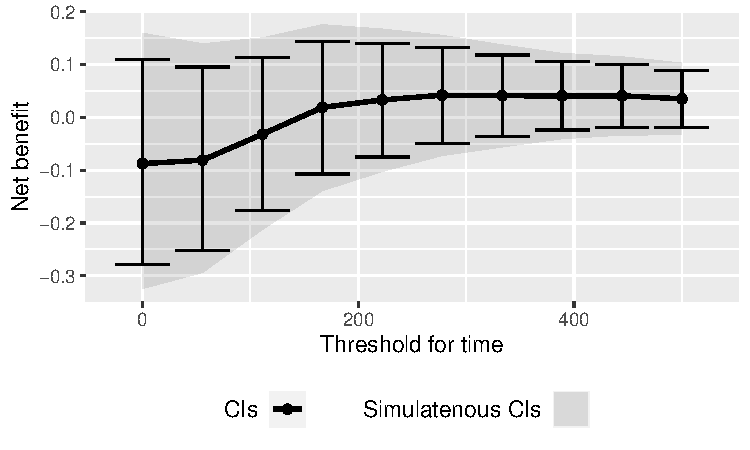
\includegraphics[width=0.5\textwidth]{./figures/gg-sensitivity1.pdf}
\end{center}

Simultaneous and pointwise confidence intervals are here of similar
width due to the very high correlation between estimates across
thresholds:
\lstset{language=r,label= ,caption= ,captionpos=b,numbers=none}
\begin{lstlisting}
BTse.cor <- cor(lava::iid(BTse.ustat))
range(BTse.cor[lower.tri(BTse.cor)])
\end{lstlisting}

\begin{verbatim}
[1] 0.3716902 0.9848999
\end{verbatim}


Note that with multiple endpoints, the thresholds can be specified using a list:
\lstset{language=r,label= ,caption= ,captionpos=b,numbers=none}
\begin{lstlisting}
BTse.H <- sensitivity(BT.H, trace = FALSE,
                      threshold = list(time = seq(0,500,length = 10), karno = c(0,40,80)))
head(BTse.H)
\end{lstlisting}

\begin{verbatim}
       time karno    estimate         se   lower.ci   upper.ci null   p.value
1   0.00000     0 -0.08754474 0.10044847 -0.2786016 0.11017738    0 0.3858987
2  55.55556     0 -0.11177487 0.09915501 -0.2995661 0.08435417    0 0.2636263
3 111.11111     0 -0.08618872 0.09822940 -0.2732475 0.10715096    0 0.3826244
4 166.66667     0 -0.05180121 0.09818252 -0.2400240 0.14017526    0 0.5984319
5 222.22222     0 -0.03668720 0.09810141 -0.2253052 0.15458146    0 0.7086747
6 277.77778     0 -0.02906324 0.09773146 -0.2172647 0.16122161    0 0.7663054
\end{verbatim}


or a matrix:

\lstset{language=r,label= ,caption= ,captionpos=b,numbers=none}
\begin{lstlisting}
grid <- expand.grid(list("time_t20" = seq(0,500,length = 10), "karno" = c(0,40,80)))
cbind(head(grid)," " = "  ...   ",tail(grid))
BTse.H2 <-sensitivity(BT.H, threshold = grid, trace = FALSE)
range(BTse.H-BTse.H2)
\end{lstlisting}

\begin{verbatim}
   time_t20 karno          time_t20 karno
1   0.00000     0   ...    222.2222    80
2  55.55556     0   ...    277.7778    80
3 111.11111     0   ...    333.3333    80
4 166.66667     0   ...    388.8889    80
5 222.22222     0   ...    444.4444    80
6 277.77778     0   ...    500.0000    80
[1] 0 0
\end{verbatim}


The latter should be used when the same endpoint is used at different
priorities (each column correspond to the threshold that should be
used at a priority). As before we can display the results using the
autoplot function:
\lstset{language=r,label= ,caption= ,captionpos=b,numbers=none}
\begin{lstlisting}
autoplot(BTse.H, col = NA)
##  alternative display:
## autoplot(BTse.H, position  = position_dodge(width = 15))
\end{lstlisting}

\begin{center}
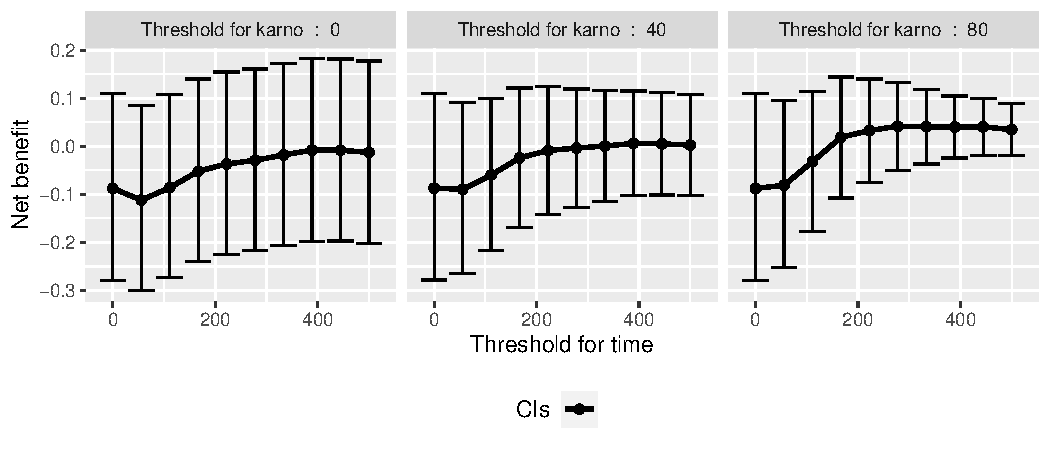
\includegraphics[width=\textwidth]{./figures/gg-sensitivity2.pdf}
\end{center}

The autoplot function can only be used when 1 or 2 thresholds are
varied at the same time.
\clearpage

\section{Getting additional inside: looking at the pair level}
\label{sec:org7243a09}

So far we have looked at the overall score and probabilities. But it
is also possible to extract the score relative to each pair, as well
as to "manually" compute this score. This can give further inside on
what the software is actually doing and what is the contribution of
each individual on the evaluation of the treatment.

\subsection{Extracting the contribution of each pair to the statistic}
\label{sec:org2a5112c}
The net treatment benefit or the win ratio statistics can be expressed as a sum
of a score over all pairs of patients. The argument \texttt{keep.pairScore}
enables to export the score relative to each pair in the output of
BuyseTest:
\lstset{language=r,label= ,caption= ,captionpos=b,numbers=none}
\begin{lstlisting}
form <- trt ~ tte(time, threshold = 20, status = "status") + cont(karno)
BT.keep <- BuyseTest(form,
                     data = veteran, keep.pairScore = TRUE, 
                     trace = 0, method.inference = "none")
\end{lstlisting}

The method \texttt{getPairScore} can then be used to extract the contribution
of each pair. For instance the following code extracts the
contribution for the first endpoint:
\lstset{language=r,label= ,caption= ,captionpos=b,numbers=none}
\begin{lstlisting}
getPairScore(BT.keep, endpoint = 1)
\end{lstlisting}

\begin{verbatim}
Key: <index.Exp, index.Pl>
      index.Pl index.Exp favorable unfavorable neutral uninf weight
         <num>     <num>     <num>       <num>   <num> <num>  <num>
   1:        1        70         1           0       0     0      1
   2:        2        70         1           0       0     0      1
   3:        3        70         1           0       0     0      1
   4:        4        70         1           0       0     0      1
   5:        5        70         1           0       0     0      1
  ---                                                              
4688:       65       137         0           1       0     0      1
4689:       66       137         0           1       0     0      1
4690:       67       137         0           1       0     0      1
4691:       68       137         0           1       0     0      1
4692:       69       137         0           1       0     0      1
\end{verbatim}

Each line corresponds to different comparison between a pair from the
control arm and the treatment arm. The column \texttt{strata} store to which
strata the pair belongs (first, second, \ldots{}). The columns favorable,
unfavorable, neutral, uninformative contains the result of the
comparison, e.g. the first pair was classified as favorable while the
last was classified as favorable with a weight of 1. The second and
third columns indicates the rows in the original dataset corresponding
to the pair:
\lstset{language=r,label= ,caption= ,captionpos=b,numbers=none}
\begin{lstlisting}
veteran[c(70,1),]
\end{lstlisting}

\begin{verbatim}
   id trt celltype time status karno diagtime age prior
70 70 Exp squamous  999      1    90       12  54    10
1   1  Pl squamous   72      1    60        7  69     0
\end{verbatim}



For the first pair, the event was observed for both observations and
since 999 > 72 + 20 the pair is rated favorable. Substracting the
average probability of the pair being favorable minus the average
probability of the pair being unfavorable:
\lstset{language=r,label= ,caption= ,captionpos=b,numbers=none}
\begin{lstlisting}
getPairScore(BT.keep, endpoint = 1)[, mean(favorable) - mean(unfavorable)]
\end{lstlisting}

\begin{verbatim}
[1] -0.08765836
\end{verbatim}


gives the net treatment benefit in favor of the treatment for the first
endpoint:
\lstset{language=r,label= ,caption= ,captionpos=b,numbers=none}
\begin{lstlisting}
BT.keep
\end{lstlisting}

\begin{verbatim}
endpoint threshold   delta   Delta
    time        20 -0.0877 -0.0877
   karno           -0.0133 -0.1009
\end{verbatim}


More examples and explanation can be found in the documentation of
the method \texttt{getPairScore}.

\subsection{Extracting the survival probabilities}
\label{sec:orga1e8820}
When using \texttt{scoring.rule} equals \texttt{"Peron"}, survival probabilities at
event time, and event times +/- threshold in the control and treatment
arms are used to score the pair. Setting \texttt{keep.survival} to \texttt{TRUE} and
\texttt{precompute} to \texttt{FALSE} in BuyseTest.options enables to export the
survival probabilities in the output of BuyseTest:
\lstset{language=r,label= ,caption= ,captionpos=b,numbers=none}
\begin{lstlisting}
BuyseTest.options(keep.survival = TRUE, precompute = FALSE)
BT.keep2 <- BuyseTest(trt ~ tte(time, threshold = 20, status = "status") + cont(karno),
                      data = veteran, keep.pairScore = TRUE, scoring.rule = "Peron",
                      trace = 0, method.inference = "none")
\end{lstlisting}

The method \texttt{getSurvival} can then be used to extract these survival
probabilities. For instance the following code extracts the survival
for the first endpoint:
\lstset{language=r,label= ,caption= ,captionpos=b,numbers=none}
\begin{lstlisting}
outSurv <- getSurvival(BT.keep2, endpoint = 1, strata = 1)
str(outSurv)
\end{lstlisting}

\begin{verbatim}
List of 5
 $ survTimeC: num [1:69, 1:13] 72 411 228 126 118 10 82 110 314 100 ...
  ..- attr(*, "dimnames")=List of 2
  .. ..$ : NULL
  .. ..$ : chr [1:13] "time" "survivalC-threshold" "survivalC_0" "survivalC+threshold" ...
 $ survTimeT: num [1:68, 1:13] 999 112 87 231 242 991 111 1 587 389 ...
  ..- attr(*, "dimnames")=List of 2
  .. ..$ : NULL
  .. ..$ : chr [1:13] "time" "survivalC-threshold" "survivalC_0" "survivalC+threshold" ...
 $ survJumpC: num [1:57, 1:6] 3 4 7 8 10 11 12 13 16 18 ...
  ..- attr(*, "dimnames")=List of 2
  .. ..$ : NULL
  .. ..$ : chr [1:6] "time" "survival" "dSurvival" "index.survival" ...
 $ survJumpT: num [1:51, 1:6] 1 2 7 8 13 15 18 19 20 21 ...
  ..- attr(*, "dimnames")=List of 2
  .. ..$ : NULL
  .. ..$ : chr [1:6] "time" "survival" "dSurvival" "index.survival" ...
 $ lastSurv : num [1:2] 0 0
\end{verbatim}

\subsubsection{Computation of the score with only one censored event}
\label{sec:org35ef0e0}

Let's look at pair 91:
\lstset{language=r,label= ,caption= ,captionpos=b,numbers=none}
\begin{lstlisting}
getPairScore(BT.keep2, endpoint = 1, rm.withinStrata = FALSE)[91]
\end{lstlisting}

\begin{verbatim}
Key: <index.Exp, index.Pl>
   index.Pl index.Exp indexWithinStrata.Pl indexWithinStrata.Exp favorable unfavorable
      <num>     <num>                <num>                 <num>     <num>       <num>
1:       22        71                   22                     2         0   0.6950827
     neutral uninf weight
       <num> <num>  <num>
1: 0.3049173     0      1
\end{verbatim}


In the dataset this corresponds to:
\lstset{language=r,label= ,caption= ,captionpos=b,numbers=none}
\begin{lstlisting}
veteran[c(22,71),]
\end{lstlisting}

\begin{verbatim}
   id trt  celltype time status karno diagtime age prior
22 22  Pl smallcell   97      0    60        5  67     0
71 71 Exp  squamous  112      1    80        6  60     0
\end{verbatim}


The observation from the control group is censored at 97 while the
observation from the treatment group has an event at 112. Since the
threshold is 20, and (112-20)<97, we know that the pair is not in
favor of the treatment. The formula for probability in favor of the
control is \(\frac{S_c(97)}{S_c(112+20)}\). The survival at the event
time in the censoring group is stored in survTimeC. Since observation
22 is the 22th observation in the control group:
\lstset{language=r,label= ,caption= ,captionpos=b,numbers=none}
\begin{lstlisting}
iSurv <- outSurv$survTimeC[22,] 
iSurv
\end{lstlisting}

\begin{verbatim}
                     time       survivalC-threshold               survivalC_0 
               97.0000000                 0.5615232                 0.5171924 
      survivalC+threshold       survivalT-threshold               survivalT_0 
                0.4235463                 0.4558824                 0.3643277 
      survivalT+threshold index.survivalC-threshold         index.survivalC_0 
                0.2827500                25.0000000                28.0000000 
index.survivalC+threshold index.survivalT-threshold         index.survivalT_0 
               33.0000000                27.0000000                32.0000000 
index.survivalT+threshold 
               35.0000000
\end{verbatim}

Since we are interested in the survival in the control arm exactly at the event time:
\lstset{language=r,label= ,caption= ,captionpos=b,numbers=none}
\begin{lstlisting}
Sc97 <- iSurv["survivalC_0"] 
Sc97
\end{lstlisting}

\begin{verbatim}
survivalC_0 
  0.5171924
\end{verbatim}


The survival at the event time in the treatment group is stored in
survTimeC. Since observation 71 is the 2nd observation in the treatment
group:
\lstset{language=r,label= ,caption= ,captionpos=b,numbers=none}
\begin{lstlisting}
iSurv <- outSurv$survTimeT[2,] ## survival at time 112+20
iSurv
\end{lstlisting}

\begin{verbatim}
                     time       survivalC-threshold               survivalC_0 
              112.0000000                 0.5319693                 0.4549201 
      survivalC+threshold       survivalT-threshold               survivalT_0 
                0.3594915                 0.3801681                 0.2827500 
      survivalT+threshold index.survivalC-threshold         index.survivalC_0 
                0.2827500                27.0000000                32.0000000 
index.survivalC+threshold index.survivalT-threshold         index.survivalT_0 
               37.0000000                31.0000000                35.0000000 
index.survivalT+threshold 
               35.0000000
\end{verbatim}

Since we are interested in the survival in the control arm at the event time plus threshold:
\lstset{language=r,label= ,caption= ,captionpos=b,numbers=none}
\begin{lstlisting}
Sc132 <- iSurv["survivalC+threshold"] 
Sc132
\end{lstlisting}

\begin{verbatim}
survivalC+threshold 
          0.3594915
\end{verbatim}


The probability in favor of the control is then:
\lstset{language=r,label= ,caption= ,captionpos=b,numbers=none}
\begin{lstlisting}
Sc132/Sc97
\end{lstlisting}

\begin{verbatim}
survivalC+threshold 
          0.6950827
\end{verbatim}

\subsubsection{Computation of the score with two censored events}
\label{sec:org7336731}

When both observations are censored, the formula for computing the
probability in favor of treatment or control involves an
integral. This integral can be computed using the function
\texttt{calcIntegralSurv\textbackslash{}\_cpp} that takes as argument a matrix containing the
survival and the jumps in survival, e.g.:
\lstset{language=r,label= ,caption= ,captionpos=b,numbers=none}
\begin{lstlisting}
head(outSurv$survJumpT)
\end{lstlisting}

\begin{verbatim}
     time  survival   dSurvival index.survival index.dsurvival1 index.dsurvival2
[1,]    1 0.7681159 -0.02941176             12                0                1
[2,]    2 0.7536232 -0.01470588             13                1                2
[3,]    7 0.7388463 -0.02941176             14                2                3
[4,]    8 0.7388463 -0.02941176             14                3                4
[5,]   13 0.7092924 -0.01470588             16                4                5
[6,]   15 0.6945155 -0.02941176             17                5                6
\end{verbatim}


and the starting time of the integration time. For instance, let's
look at pair 148:
\lstset{language=r,label= ,caption= ,captionpos=b,numbers=none}
\begin{lstlisting}
getPairScore(BT.keep2, endpoint = 1, rm.withinStrata = FALSE)[148]
\end{lstlisting}

\begin{verbatim}
Key: <index.Exp, index.Pl>
   index.Pl index.Exp indexWithinStrata.Pl indexWithinStrata.Exp favorable unfavorable
      <num>     <num>                <num>                 <num>     <num>       <num>
1:       10        72                   10                     3 0.5058685   0.3770426
     neutral uninf weight
       <num> <num>  <num>
1: 0.1170889     0      1
\end{verbatim}


which corresponds to the observations:
\lstset{language=r,label= ,caption= ,captionpos=b,numbers=none}
\begin{lstlisting}
veteran[c(10,72),]
\end{lstlisting}

\begin{verbatim}
   id trt celltype time status karno diagtime age prior
10 10  Pl squamous  100      0    70        6  70     0
72 72 Exp squamous   87      0    80        3  48     0
\end{verbatim}


The probability in favor of the treatment (\(p_F\)) and control (\(p_{UF}\)) can be computed
as:
\begin{align*}
p_F &= -\frac{1}{S_T(x)S_C(y)}\int_{t>y} S_T(t+\tau) dS_C(t) \\
p_{UF} &= -\frac{1}{S_T(x)S_C(y)}\int_{t>x} S_C(t+\tau) dS_T(t)
\end{align*}
where \(x=87\) and \(y=100\). To ease the call of \texttt{calcIntegralScore\_cpp} we create a warper:
\lstset{language=r,label= ,caption= ,captionpos=b,numbers=none}
\begin{lstlisting}
calcInt <- function(...){ ## no need for the functionnal derivative of the score 
    BuyseTest:::.calcIntegralSurv_cpp(..., 
                                      returnDeriv = FALSE, 
                                      derivSurv = matrix(0), 
                                      derivSurvD = matrix(0))
}
\end{lstlisting}

\clearpage

and then call it to compute the probabilities:
\lstset{language=r,label= ,caption= ,captionpos=b,numbers=none}
\begin{lstlisting}
denom <- as.double(outSurv$survTimeT[3,"survivalT_0"] * outSurv$survTimeC[10,"survivalC_0"])
M <- cbind("favorable" = -calcInt(outSurv$survJumpC, start = 100, 
                                  lastSurv = outSurv$lastSurv[2],
                                  lastdSurv = outSurv$lastSurv[1])/denom,
           "unfavorable" = -calcInt(outSurv$survJumpT, start = 87, 
                                    lastSurv = outSurv$lastSurv[1],
                                    lastdSurv = outSurv$lastSurv[2])/denom)
rownames(M) <- c("lowerBound","upperBound")
M
\end{lstlisting}

\begin{verbatim}
           favorable unfavorable
lowerBound 0.5058685   0.3770426
upperBound 0.5058685   0.3770426
\end{verbatim}


Note: the lower bound is identical to the upper bound as we could
estimate the full survival curve:
\lstset{language=r,label= ,caption= ,captionpos=b,numbers=none}
\begin{lstlisting}
outSurv$lastSurv
\end{lstlisting}

\begin{verbatim}
[1] 0 0
\end{verbatim}


\clearpage

\section{Dealing with missing values or/and right censoring}
\label{sec:org763d7c3}

In presence of censoring or missing values, it is often not be
 possible to classify all pairs without a model for the censoring
 mechanism. The unclassified pairs, called uninformative, have a score
 of 0 which will typically bias the estimate of the net net treatment benefit
 towards 0 \footnote{While the power is typically reduced, the type 1 error
 will still be controled if censoring is at random}. Consider the
 following dataset:
\lstset{language=r,label= ,caption= ,captionpos=b,numbers=none}
\begin{lstlisting}
set.seed(10)
dt <- simBuyseTest(1e2, latent = TRUE, argsCont = NULL,
                   argsTTE = list(scale.T = 1/2, scale.C = 1,
                                  scale.censoring.C = 1, scale.censoring.T = 1))
dt[, eventtimeCensoring := NULL]
dt[, status1 := 1]
head(dt)
\end{lstlisting}

\begin{verbatim}
      id treatment eventtimeUncensored eventtime status toxicity eta_toxicity status1
   <num>    <fctr>               <num>     <num>  <num>   <fctr>        <num>   <num>
1:     1         C           0.2135567 0.2135567      1      yes  -0.07945702       1
2:     2         C           0.3422379 0.3422379      1       no   1.18175155       1
3:     3         C           1.3933222 1.3933222      1       no   2.18614406       1
4:     4         C           0.6737702 0.1961599      0       no   0.40617493       1
5:     5         C           0.5642992 0.5642992      1      yes  -0.73835910       1
6:     6         C           1.1039218 0.1764950      0      yes  -1.95648670       1
\end{verbatim}


where we have the uncensored event times (\texttt{eventtimeUncensored}) as well as the censored event
times (\texttt{eventtime}). The percentage of censored observations is:
\lstset{language=r,label= ,caption= ,captionpos=b,numbers=none}
\begin{lstlisting}
100*dt[,mean(status==0)]
\end{lstlisting}

\begin{verbatim}
[1] 44
\end{verbatim}


We would like to be able to recover the net treatment benefit estimated with the uncensored event times:
\lstset{language=r,label= ,caption= ,captionpos=b,numbers=none}
\begin{lstlisting}
BuyseTest(treatment ~ tte(eventtimeUncensored, status1, threshold = 0.5),
          data = dt,
          scoring.rule = "Gehan", method.inference = "none", trace = 0)
\end{lstlisting}

\begin{verbatim}
           endpoint threshold  Delta
eventtimeUncensored       0.5 -0.271
\end{verbatim}


using the censored survival times.

\clearpage

The \texttt{BuyseTest} function handles missing values via two arguments:
\begin{itemize}
\item \texttt{scoring.rule} indicates how pairs involving missing data are compared. 
\begin{itemize}
\item \textbf{the Gehan's scoring rule} compares the observed values. If it is
not possible to decide whether one observation has a better
endpoint than the other (e.g. because both are right-censoring)
then the paired is scored uninformative.
\item \textbf{the Peron's scoring rule} compares the probabilty of one
observation having a better endpoint than the other given the
observed values. This require a model for the censoring
distribution. If the full survival curve can be identified then
all pairs can be fully classified otherwise some of the pair
will be partially uninformative.
\item \textbf{the Efron's scoring rule} same as the Peron's scoring rule
except that the survival curve is extrapolated to 0 when its
tail is unknown. Only relevant when using a (stratified)
Kaplan-Meier estimator and no competing risks.
\end{itemize}
\item \texttt{correction.uninf} indicates what to do with the uninformative
scores. For instance setting this argument to \texttt{TRUE} will
re-distribute this score to favorable/unfavorable/neutral scores.
\end{itemize}

The Peron's scoring rule is the default (and recommanded) approach. It
uses a Kaplan Meier estimator stratified on treatment and GPC \texttt{strata}
variable (if any) as survival model. When the last observation is
censored, then part of the survival curve is unknown which can be
necessary to score some of the pairs (especially in presence of a
threshold of clinical relevance). One can:
\begin{itemize}
\item use a restriction time within the time interval where the survival
curve can be estimated for each group.
\item still use the default Peron's scoring rule: this will lead to
uninformative pairs which can be re-classified based on a lower
priority endpoint.
\item use the Peron's scoring rule with another survival model, using
parametric assumptions to inform about the unknown part of the
survival curve. This can be achieved via the \texttt{model.tte} argument or
using the Efron's scoring rule.
\item use an add-hoc correction for the uninformative pairs
(\texttt{correction.uninf})
\end{itemize}

The first two solutions lead to a change of estimand, the first being
much more clearly defined than the second. The last two solutions
correspond to make statistical assumptions, the former assumptions
being more explicit than with the later solution.

\subsection{Gehan's scoring rule}
\label{sec:orgf9002db}
In the example, Gehan's scoring rule:
\lstset{language=r,label= ,caption= ,captionpos=b,numbers=none}
\begin{lstlisting}
e.G <- BuyseTest(treatment ~ tte(eventtime, status, threshold = 0.5),
          data = dt, scoring.rule = "Gehan", trace = 0)
model.tables(e.G)
\end{lstlisting}

\begin{verbatim}
   endpoint threshold total favorable unfavorable neutral uninf   Delta   lower.ci
1 eventtime       0.5   100      4.67       14.39   20.44  60.5 -0.0972 -0.1593869
     upper.ci     p.value
1 -0.03424474 0.002514882
\end{verbatim}


leads to many uninformative pairs (about 60\%) and an estimate much
closer to 0 than the truth.

\subsection{Peron's scoring rule}
\label{sec:orge82fd83}
In the example, Peron's scoring rule:
\lstset{language=r,label= ,caption= ,captionpos=b,numbers=none}
\begin{lstlisting}
e.P <- BuyseTest(treatment ~ tte(eventtime, status, threshold = 0.5),
          data = dt, scoring.rule = "Peron", trace = 0)
model.tables(e.P)
\end{lstlisting}

\begin{verbatim}
   endpoint threshold total favorable unfavorable  neutral    uninf      Delta   lower.ci
1 eventtime       0.5   100   11.1737    43.33707 44.12373 1.365504 -0.3216337 -0.4584262
    upper.ci      p.value
1 -0.1699543 5.385074e-05
\end{verbatim}


leads to no uninformative pairs. Indeed the last observation in each
group is an (uncensored) event:
\lstset{language=r,label= ,caption= ,captionpos=b,numbers=none}
\begin{lstlisting}
dt[,.SD[which.max(eventtime)],by="treatment"]
\end{lstlisting}

\begin{verbatim}
   treatment    id eventtimeUncensored eventtime status toxicity eta_toxicity status1
      <fctr> <num>               <num>     <num>  <num>   <fctr>        <num>   <num>
1:         C    72            2.668629  2.668629      1      yes   -1.9256436       1
2:         T   154            1.674053  1.588657      0      yes   -0.8647272       1
\end{verbatim}

so the full survival curve could be identified. As a result the estimate is very close to the
truth. 

\bigskip

\noindent \uline{Note 1:} the censoring model can be specified by first fitting a
survival model (\texttt{prodlim} or \texttt{survreg}) for the survival time:
\lstset{language=r,label= ,caption= ,captionpos=b,numbers=none}
\begin{lstlisting}
library(prodlim)
e.prodlim <- prodlim(Hist(eventtime, status) ~ treatment, data = dt)
\end{lstlisting}

Then passing the model to the \texttt{BuyseTest} via the \texttt{model.tte} argument:
\lstset{language=r,label= ,caption= ,captionpos=b,numbers=none}
\begin{lstlisting}
e.P1 <- BuyseTest(treatment ~ tte(eventtime, status, threshold = 0.5),
                  model.tte = e.prodlim,
                  data = dt, scoring.rule = "Peron", trace = 0)
model.tables(e.P1)
\end{lstlisting}

\begin{verbatim}
   endpoint threshold total favorable unfavorable  neutral    uninf      Delta   lower.ci
1 eventtime       0.5   100   11.1737    43.33707 44.12373 1.365504 -0.3216337 -0.4584262
    upper.ci      p.value
1 -0.1699543 5.385074e-05
\end{verbatim}


When the dataset used to fit the survival model match the one used to
run the GPC procedure, the overall uncertainty will be
computed. Otherwise:
\lstset{language=r,label= ,caption= ,captionpos=b,numbers=none}
\begin{lstlisting}
dt2 <- dt[order(dt$eventtime)]
e.P2 <- BuyseTest(treatment ~ tte(eventtime, status, threshold = 0.5),
                  model.tte = prodlim(Hist(eventtime, status) ~ treatment, data = dt2),
                  data = dt, scoring.rule = "Peron", trace = 0)
model.tables(e.P2)
\end{lstlisting}

\begin{verbatim}
Uncertainty related to the estimation of the survival probabilities is ignored. 
Consider adding an attribute "iidNuisance" to the argument 'model.tte' taking value TRUE to change this default behavior.
   endpoint threshold total favorable unfavorable  neutral    uninf      Delta   lower.ci
1 eventtime       0.5   100   11.1737    43.33707 44.12373 1.365504 -0.3216337 -0.4187087
    upper.ci      p.value
1 -0.2172912 6.570106e-09
\end{verbatim}


the survival probabilities will assumed to be known with infinite
precision and only the uncertainty of the GPC procedure will be
considered. Add-hoc modification of the data can be used to obtain
'conservative' estimates when considering a single endpoint, e.g.:
\lstset{language=r,label= ,caption= ,captionpos=b,numbers=none}
\begin{lstlisting}
dt2[, last := (max(eventtime)==eventtime), by = "treatment"]
## survival stays constant after end of follow-up
dt2[treatment=="C" & last == TRUE, c("eventtime","status") := .(max(dt2$eventtime)+1,1)]
## survival drop to 0 after end of follow-up
dt2[treatment=="T" & last == TRUE, status := 1]
## modified Kaplan Meier estimator
e.prodlim2 <- prodlim(Hist(eventtime, status) ~ treatment, data = dt2)
attr(e.prodlim2, "iidNuisance") <- TRUE
## run GPC
e.P3 <- BuyseTest(treatment ~ tte(eventtime, status, threshold = 0.5),
                  model.tte = e.prodlim2,
                  data = dt, scoring.rule = "Peron", trace = 0)
model.tables(e.P3) ## even more unfavorable to treatment
\end{lstlisting}

\begin{verbatim}
   endpoint threshold total favorable unfavorable  neutral uninf      Delta   lower.ci
1 eventtime       0.5   100   11.1737    43.97856 44.84774     0 -0.3280486 -0.4378751
    upper.ci     p.value
1 -0.2085751 2.25273e-07
\end{verbatim}


\bigskip

\uline{Note 2:} it is possible to use a parametric model via the \texttt{survreg} function:
\lstset{language=r,label= ,caption= ,captionpos=b,numbers=none}
\begin{lstlisting}
library(survival)
e.survreg <- survreg(Surv(eventtime, status) ~ treatment, data = dt, 
                     dist = "weibull")
\end{lstlisting}

Then passing the model to the \texttt{BuyseTest} via the \texttt{model.tte} argument:
\lstset{language=r,label= ,caption= ,captionpos=b,numbers=none}
\begin{lstlisting}
e.P3 <- BuyseTest(treatment ~ tte(eventtime, status, threshold = 0.5),
                  model.tte = e.survreg,
                  data = dt, scoring.rule = "Peron", trace = 0)
model.tables(e.P3)
\end{lstlisting}
\begin{verbatim}
   endpoint threshold total favorable unfavorable  neutral      uninf      Delta   lower.ci
1 eventtime       0.5   100  11.65444    34.18937 54.14472 0.01147085 -0.2253494 -0.3476693
     upper.ci      p.value
1 -0.09548719 0.0007624659
\end{verbatim}


Internally the survival curve is discretized using 1000 points
starting from survival = 1 to survival = 0.001 (this is why there is a
non-0 but small percentage of uninformative pairs). This is performed
internally by applying the \texttt{BuyseTTEM} method. Another discretisation
can be obtained by calling \texttt{BuyseTTEM} with another value for the \texttt{n.grid} argument:
\lstset{language=r,label= ,caption= ,captionpos=b,numbers=none}
\begin{lstlisting}
e.TTEM <- BuyseTTEM(e.survreg, treatment = "treatment", iid = TRUE, n.grid = 2500)
str(e.TTEM$peron$jumpSurvHaz[[1]][[1]])
\end{lstlisting}

\begin{verbatim}
'data.frame':	2500 obs. of  3 variables:
 $ index.jump: logi  NA NA NA NA NA NA ...
 $ time.jump : num  0 0.000307 0.000632 0.000964 0.001301 ...
 $ survival  : num  1 1 0.999 0.999 0.998 ...
\end{verbatim}


and then passing to \texttt{BuyseTest}:
\lstset{language=r,label= ,caption= ,captionpos=b,numbers=none}
\begin{lstlisting}
e.P4 <- BuyseTest(treatment ~ tte(eventtime, status, threshold = 0.5),
                  model.tte = e.TTEM,
                  data = dt, scoring.rule = "Peron", trace = 0)
model.tables(e.P4)
\end{lstlisting}

\begin{verbatim}
   endpoint threshold total favorable unfavorable  neutral       uninf      Delta   lower.ci
1 eventtime       0.5   100  11.64894    34.18631 54.16019 0.004558007 -0.2253737 -0.3476861
     upper.ci      p.value
1 -0.09551899 0.0007609754
\end{verbatim}


It is therefore possible to extend the approach to other model by
defining an appropriate \texttt{BuyseTTEM} method. Looking at the code use
for defining \texttt{BuyseTTEM.survreg} can be helpful.

\subsection{Correction via re-weighting}
\label{sec:org00db701}

The weights of the non-informative pairs is redistributed
to the informative pairs. This is only a good strategy when there are
no neutral pairs or there are no lower priority endpoints. This gives
an estimate much closer to the true net treatment benefit:
\lstset{language=r,label= ,caption= ,captionpos=b,numbers=none}
\begin{lstlisting}
BT <- BuyseTest(treatment ~ tte(eventtime, status, threshold = 0.5),
                data = dt, keep.pairScore = TRUE, trace = 0,
                scoring.rule = "Gehan", method.inference = "none", correction.uninf = 2)
summary(BT)
\end{lstlisting}

\begin{verbatim}
      Generalized pairwise comparisons with 1 endpoint

- statistic       : net treatment benefit  (delta: endpoint specific, Delta: global) 
- treatment groups: T (treatment) vs. C (control) 
- censored pairs  : deterministic score or uninformative
- uninformative pairs: no contribution, their weight is passed to the informative pairs using IPCW
- results
 endpoint threshold total(%) favorable(%) unfavorable(%) neutral(%) uninf(%)   Delta
eventtime       0.5      100        11.82          36.43      51.75        0 -0.2461
\end{verbatim}



We can also see that no pair is finally classified as non
informative. To get some inside about the correction we can look at
the scores of the pairs:
\lstset{language=r,label= ,caption= ,captionpos=b,numbers=none}
\begin{lstlisting}
iScore <- getPairScore(BT, endpoint = 1)
\end{lstlisting}

To get a synthetic view, we only look at the unique
favorable/unfavorable/neutral/uniformative results:
\lstset{language=r,label= ,caption= ,captionpos=b,numbers=none}
\begin{lstlisting}
iScore[,.SD[1], 
       .SDcols = c("favorableC","unfavorableC","neutralC","uninfC"),
       by = c("favorable","unfavorable","neutral","uninf")]
\end{lstlisting}

\begin{verbatim}
   favorable unfavorable neutral uninf favorableC unfavorableC neutralC uninfC
       <num>       <num>   <num> <num>      <num>        <num>    <num>  <num>
1:         0           0       1     0   0.000000     0.000000 2.531646      0
2:         0           1       0     0   0.000000     2.531646 0.000000      0
3:         0           0       0     1   0.000000     0.000000 0.000000      0
4:         1           0       0     0   2.531646     0.000000 0.000000      0
\end{verbatim}


We can see that the favorable/unfavorable/neutral pairs have seen
their contribution multiplied by:
\lstset{language=r,label= ,caption= ,captionpos=b,numbers=none}
\begin{lstlisting}
iScore[,1/mean(favorable + unfavorable + neutral)]
\end{lstlisting}

\begin{verbatim}
[1] 2.531646
\end{verbatim}


i.e. the inverse probability of being informative. 

\subsection{Correction at the pair level}
\label{sec:org28d3aaf}

Another possible correction is to distribute the non-informative
weight of a pair to the average favorable/unfavorable/neutral
probability observed on the sample:
\lstset{language=r,label= ,caption= ,captionpos=b,numbers=none}
\begin{lstlisting}
BT <- BuyseTest(treatment ~ tte(eventtime, status, threshold = 0.5),
                data = dt, keep.pairScore = TRUE, trace = 0,
                scoring.rule = "Gehan", method.inference = "none", correction.uninf = TRUE)
summary(BT)
\end{lstlisting}

\begin{verbatim}
      Generalized pairwise comparisons with 1 endpoint

- statistic       : net treatment benefit  (delta: endpoint specific, Delta: global) 
- treatment groups: T (treatment) vs. C (control) 
- censored pairs  : deterministic score or uninformative
- uninformative pairs: score equals the averaged score of all informative pairs
- results
 endpoint threshold total(%) favorable(%) unfavorable(%) neutral(%) uninf(%)   Delta
eventtime       0.5      100        11.82          36.43      51.75        0 -0.2461
\end{verbatim}



Looking at the scores of the pairs:
\lstset{language=r,label= ,caption= ,captionpos=b,numbers=none}
\begin{lstlisting}
iScore <- getPairScore(BT, endpoint = 1)
iScore[,.SD[1], 
       .SDcols = c("favorableC","unfavorableC","neutralC","uninfC"),
       by = c("favorable","unfavorable","neutral","uninf")]
\end{lstlisting}

\begin{verbatim}
   favorable unfavorable neutral uninf favorableC unfavorableC  neutralC uninfC
       <num>       <num>   <num> <num>      <num>        <num>     <num>  <num>
1:         0           0       1     0  0.0000000    0.0000000 1.0000000      0
2:         0           1       0     0  0.0000000    1.0000000 0.0000000      0
3:         0           0       0     1  0.1182278    0.3643038 0.5174684      0
4:         1           0       0     0  1.0000000    0.0000000 0.0000000      0
\end{verbatim}


we can see that the corrected probability have not changed for the
informative pairs, but for the non-informative they have been set to:
\lstset{language=r,label= ,caption= ,captionpos=b,numbers=none}
\begin{lstlisting}
iScore[, .(favorable = weighted.mean(favorable, w = 1-uninf), 
           unfavorable = weighted.mean(unfavorable, w = 1-uninf), 
           neutral = weighted.mean(neutral, w = 1-uninf))]
\end{lstlisting}

\begin{verbatim}
   favorable unfavorable   neutral
       <num>       <num>     <num>
1: 0.1182278   0.3643038 0.5174684
\end{verbatim}

\subsection{Note on the use of the corrections}
\label{sec:org642010c}

As mentioned in \cite{peron2021correcting}, the corrections (at the pair
level or IPCW) are assumes that uninformative pairs would on average
behave like informative pairs. This is typically the case under the
proportional hazard assumption. However that may not be the case with
other distributions, e.g.:
\lstset{language=r,label= ,caption= ,captionpos=b,numbers=none}
\begin{lstlisting}
set.seed(10);n <- 250; 
df <- rbind(data.frame(group = "T1", time = rweibull(n, shape = 1, scale = 2), status = 1),
            data.frame(group = "T2", time = rweibull(n, shape = 2, scale = 1.8), status = 1))
df$censoring <- runif(NROW(df),0,2)
df$timeC <- pmin(df$time,df$censoring)
df$statusC <- as.numeric(df$time<=df$censoring)
plot(prodlim(Hist(time,status)~group, data = df)); title("complete data");
plot(prodlim(Hist(timeC,statusC)~group, data = df)); title("right-censored data");
\end{lstlisting}
\begin{center}
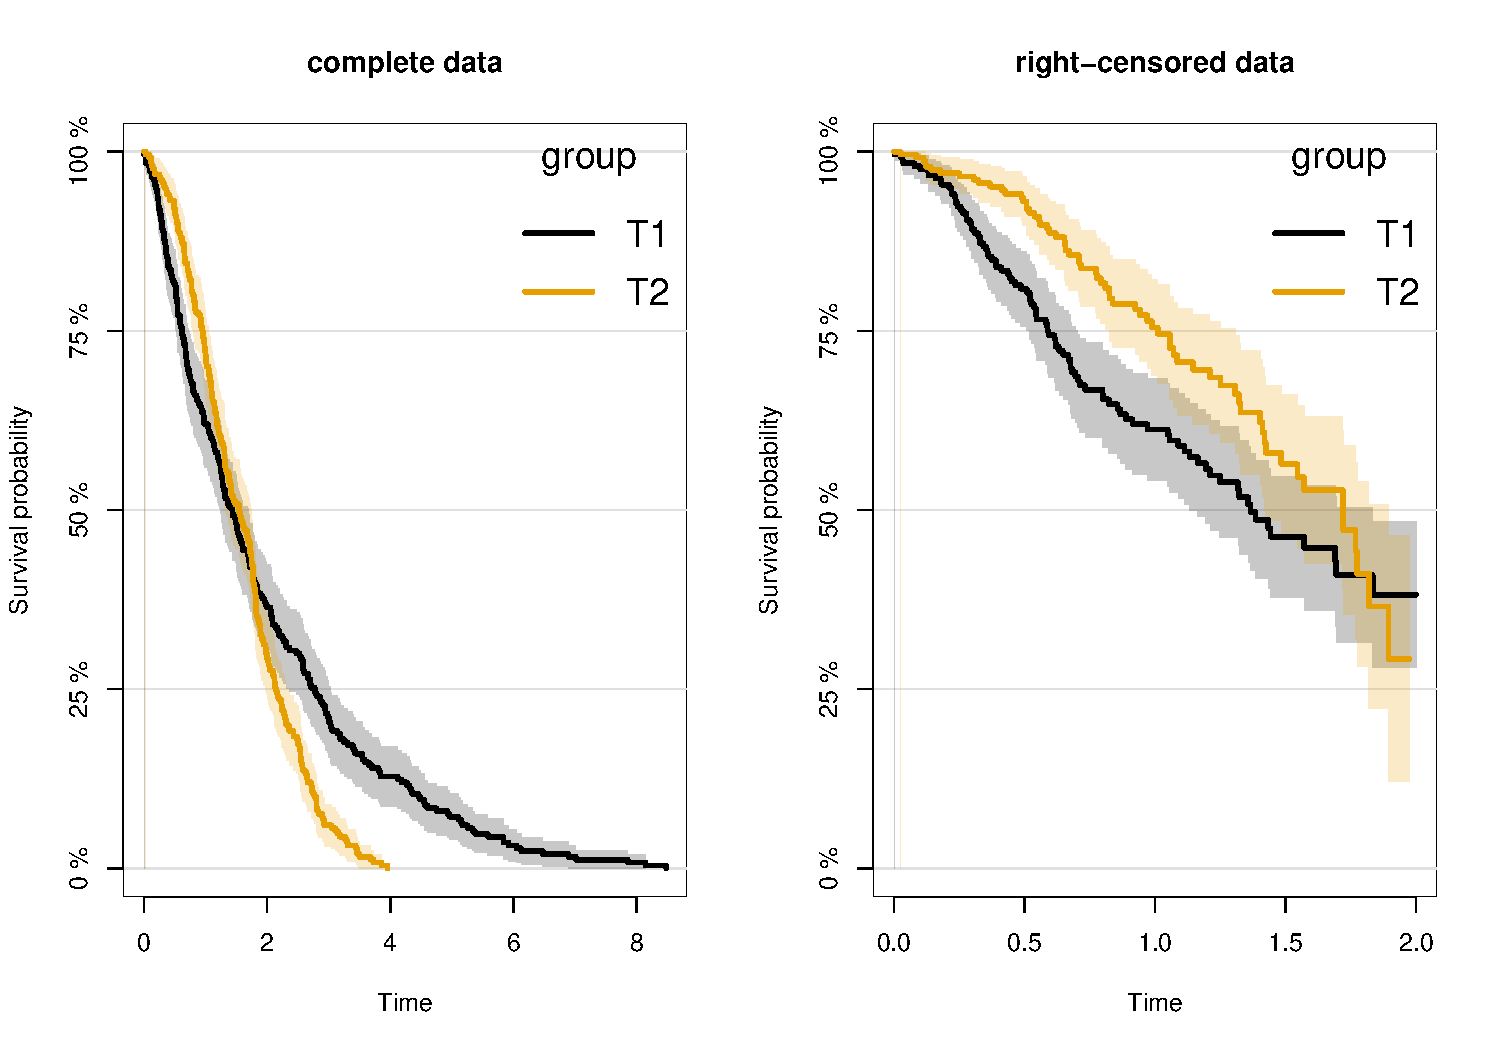
\includegraphics[width=0.8\textwidth]{./figures/plot-crossingSurv.pdf}
\end{center}

Here the net treatment benefit that we would have estimated with complete data:
\lstset{language=r,label= ,caption= ,captionpos=b,numbers=none}
\begin{lstlisting}
BuyseTest.options(method.inference = "none")
e.ref <- BuyseTest(group ~ tte(time,status), data = df, trace = FALSE)
s.ref <- model.tables(e.ref, column = c("favorable","unfavorable","neutral","uninf","Delta"))
s.ref
\end{lstlisting}

\begin{verbatim}
  favorable unfavorable neutral uninf    Delta
1   50.2048     49.7952       0     0 0.004096
\end{verbatim}


can be taken as a reference. Violation of the assumption will in this
example have a substantial impact and lead to a worse estimate with
the correction:
\lstset{language=r,label= ,caption= ,captionpos=b,numbers=none}
\begin{lstlisting}
e.correction <- BuyseTest(group ~ tte(timeC,statusC), data = df, trace = FALSE, correction.uninf = TRUE)
s.correction <- model.tables(e.correction, column = c("favorable","unfavorable","neutral","uninf","Delta"))
\end{lstlisting}

\begin{verbatim}
Warning message:
In .BuyseTest(envir = envirBT, iid = outArgs$iid, method.inference = "none",  :
  Some of the survival curves for endpoint(s) "timeC" are unknown beyond a survival of 0.25.
The correction of uninformative pairs assume that uninformative pairs would on average behave like informative pairs. 
This can be a strong assumption and have substantial impact when the tail of the survival curve is unknown.
\end{verbatim}


than without:
\lstset{language=r,label= ,caption= ,captionpos=b,numbers=none}
\begin{lstlisting}
e.Peron <- BuyseTest(group ~ tte(timeC,statusC), data = df, trace = FALSE)
s.Peron <- model.tables(e.Peron, column = c("favorable","unfavorable","neutral","uninf","Delta"))
rbind("reference" = s.ref,
      "no correction" = s.Peron,
      "correction" = s.correction)
\end{lstlisting}
\begin{verbatim}
              favorable unfavorable neutral    uninf      Delta
reference      50.20480    49.79520       0  0.00000 0.00409600
no correction  49.09253    39.74775       0 11.15972 0.09344778
correction     55.25931    44.74069       0  0.00000 0.10518628
\end{verbatim}


\clearpage

\section{Simulating data using \texttt{simBuyseTest}}
\label{sec:orgcc30d44}
You can simulate data with the \texttt{simBuyseTest} function. For instance
the following code simulates data for 5 individuals in the treatment
arm and 5 individuals in the control arm:
\lstset{language=r,label= ,caption= ,captionpos=b,numbers=none}
\begin{lstlisting}
set.seed(10)
simBuyseTest(n.T = 5, n.C = 5)
\end{lstlisting}

\begin{verbatim}
       id treatment  eventtime status toxicity       score
    <int>    <fctr>      <num>  <num>   <fctr>       <num>
 1:     1         C 0.60539304      0      yes -1.85374045
 2:     2         C 0.31328027      1      yes -0.07794607
 3:     3         C 0.03946623      0      yes  0.96856634
 4:     4         C 0.32147489      1      yes  0.18492596
 5:     5         C 1.57044952      0      yes -1.37994358
 6:     6         T 0.29069131      0       no  1.10177950
 7:     7         T 0.19522131      0      yes  0.75578151
 8:     8         T 0.04640668      0      yes -0.23823356
 9:     9         T 0.05277335      1      yes  0.98744470
10:    10         T 0.43062009      1      yes  0.74139013
\end{verbatim}

By default a categorical, continuous and time to event outcome are
generated independently. You can modify their distribution via the
arguments \texttt{argsBin}, \texttt{argsCont}, \texttt{argsTTE}. For instance the following
code simulates two continuous variables with mean 5 in the treatment
arm and 10 in the control arm all with variance 1:
\lstset{language=r,label= ,caption= ,captionpos=b,numbers=none}
\begin{lstlisting}
set.seed(10)
argsCont <- list(mu.T = c(5,5), mu.C = c(10,10), 
                 sigma.T = c(1,1), sigma.C = c(1,1),
                 name = c("tumorSize","score"))
dt <- simBuyseTest(n.T = 5, n.C = 5,
                   argsCont = argsCont)
dt
\end{lstlisting}

\begin{verbatim}
       id treatment eventtime status toxicity tumorSize     score
    <int>    <fctr>     <num>  <num>   <fctr>     <num>     <num>
 1:     1         C 0.1805891      0      yes 11.086551  8.564486
 2:     2         C 0.1702538      1      yes  9.237455 10.362087
 3:     3         C 0.2621793      1       no  9.171337  8.240913
 4:     4         C 0.2959301      0       no 10.834474  9.675456
 5:     5         C 0.4816549      1      yes  9.032348  9.348437
 6:     6         T 0.6446131      1       no  5.089347  6.101780
 7:     7         T 0.7372264      1      yes  4.045056  5.755782
 8:     8         T 0.7213402      0      yes  4.804850  4.761766
 9:     9         T 0.1580651      1      yes  5.925521  5.987445
10:    10         T 0.2212117      0      yes  5.482979  5.741390
\end{verbatim}

This functionality is based on the \texttt{sim} function of the \textbf{lava}
package.

\clearpage

\section{Power calculation using \texttt{powerBuyseTest}}
\label{sec:org786855f}

The function \texttt{powerBuyseTest} can be used to perform power
calculation, i.e., estimate the probability of rejecting a null
hypothesis under a specific generative mechanism. The user therefore
need to specify:
\begin{itemize}
\item the generative mechanism via a function \hfill \textcolor{orange}{- argument \texttt{sim}}
\item the null hypothesis \hfill \textcolor{orange}{- argument \texttt{null}}
\item the sample size(s) for the which the power should be computed  \hfill \textcolor{orange}{- argument \texttt{sample.size}}
\end{itemize}

\bigskip

Consider the following generative mechanism where the outcome follows
a Student's t-distribution in the treatment and control group, with same
variance and degrees of freedom but different mean:
\lstset{language=r,label= ,caption= ,captionpos=b,numbers=none}
\begin{lstlisting}
simFCT <- function(n.C, n.T){
     out <- rbind(cbind(Y=stats::rt(n.C, df = 5), group=0),
                  cbind(Y=stats::rt(n.T, df = 5) + 1/2, group=1))
     return(data.table::as.data.table(out))
}
set.seed(10)
simFCT(101,101)
\end{lstlisting}

\begin{verbatim}
               Y group
           <num> <num>
  1:  0.02241932     0
  2: -1.07273566     0
  3:  0.76072274     0
  4: -0.25812356     0
  5:  0.97207866     0
 ---                  
198:  1.82349375     1
199: -0.98560076     1
200:  1.48143637     1
201:  3.69314316     1
202:  0.96244416     1
\end{verbatim}

We then define the null hypothesis:
\lstset{language=r,label= ,caption= ,captionpos=b,numbers=none}
\begin{lstlisting}
null <- c("netBenefit" = 0)
\end{lstlisting}

Naming the value is important since that will indicate which statistic
should be used (here the net treatment benefit). We can assess the power of a
test based on the net treatment benefit using the following syntax:
\lstset{language=r,label= ,caption= ,captionpos=b,numbers=none}
\begin{lstlisting}
powerW <- powerBuyseTest(sim = simFCT, method.inference = "u-statistic", null = null,
                         sample.size = c(5,10,20,30,50,100),                         
                         formula = group ~ cont(Y), 
                         n.rep = 1000, seed = 10, cpus = 6, trace = 0)
\end{lstlisting}

\clearpage

And use the summary method to display the power (column
\texttt{rejection.rate}):
\lstset{language=r,label= ,caption= ,captionpos=b,numbers=none}
\begin{lstlisting}
summary(powerW)
\end{lstlisting}

\begin{verbatim}
        Simulation study with Generalized pairwise comparison
        with 1000 samples

 - net benefit statistic (null hypothesis Delta=0)
 endpoint threshold n.T n.C mean.estimate sd.estimate mean.se rejection.rate
        Y     1e-12   5   5        0.2484       0.359  0.3395          0.069
                     10  10        0.2471      0.2551  0.2464          0.137
                     20  20        0.2444      0.1746  0.1757          0.221
                     30  30         0.243      0.1436  0.1437          0.365
                     50  50        0.2438      0.1114  0.1113          0.557
                    100 100        0.2458      0.0804  0.0787          0.865

 n.T          : number of observations in the treatment group
 n.C          : number of observations in the control group
 mean.estimate: average estimate over simulations
 sd.estimate  : standard deviation of the estimate over simulations
 mean.se      : average estimated standard error of the estimate over simulations
 rejection    : frequency of the rejection of the null hypothesis over simulations
(standard error: H-projection of order 1| p-value: after transformation)
\end{verbatim}

It is also possibly to use an asymptotic approximation to derive a
approximate sample size satisfying a specific type 1 and type 2 error
rate:
\lstset{language=r,label= ,caption= ,captionpos=b,numbers=none}
\begin{lstlisting}
nW <- powerBuyseTest(sim = simFCT, method.inference = "u-statistic", 
                     power = 0.8, max.sample.size = 1000,                     
                     formula = group ~ cont(Y), null = c("netBenefit" = 0),
                     n.rep = c(1000,10), seed = 10, cpus = 5, trace = 0)
\end{lstlisting}

This procedure is inspired from the procedure presented by
\cite{brunner2018rank} in section 3.8.2.2. In short, several 'large'
datasets are generated and analyzed using GPC to approximate the
statistic of interest (\(\Delta\)) and its asymptotic variance
(\(\sigma^2\)). The sample size needed to achieve the requested power
(\(1-\beta\)) and the requested type 1 error (\(\alpha\)) is then
deduce, give a dataset, according to the equation \(N = \sigma^2
\frac{\left(u_{1-\alpha/2}+u_{1-\beta}\right)^2}{\Delta^2}\) where
\(u_x\) denotes the x-quantile of the normal distribution. The
estimated sample size is then the average calculated sample size
across dataset. The argument \texttt{max.sample.size} specifies the number of
observation per group in the 'large' dataset (here 1000 per group) and
the second element of the argument \texttt{n.rep} specifies the number of
datasets (here 10). The quality of the approximation, as well as the
computation time, thus improves when increasing \texttt{max.sample.size} and
\texttt{n.rep[2]}. The achieved power with the estimated sample size can be
output as usual using the \texttt{summary} method:
\lstset{language=r,label= ,caption= ,captionpos=b,numbers=none}
\begin{lstlisting}
summary(nW)
\end{lstlisting}

\begin{verbatim}
        Sample size calculation with Generalized pairwise comparison
        for a power of 0.8 and type 1 error rate of 0.05 

 - estimated sample size (mean [min;max]): 89 [60;145] controls
                                           89 [60;145] treated

 - net benefit statistic (null hypothesis Delta=0)
 endpoint threshold n.T n.C mean.estimate sd.estimate mean.se rejection.rate
        Y     1e-12  89  89        0.2452      0.0854  0.0834          0.806

 n.T          : number of observations in the treatment group
 n.C          : number of observations in the control group
 mean.estimate: average estimate over simulations
 sd.estimate  : standard deviation of the estimate over simulations
 mean.se      : average estimated standard error of the estimate over simulations
 rejection    : frequency of the rejection of the null hypothesis over simulations
(standard error: H-projection of order 1| p-value: after transformation)
\end{verbatim}

\clearpage

\section{Modifying default options}
\label{sec:orga4fbd92}
The \texttt{BuyseTest.options} method enable to get and set the default
options of the \texttt{BuyseTest} function. For instance, the default option
for trace is:
\lstset{language=r,label= ,caption= ,captionpos=b,numbers=none}
\begin{lstlisting}
BuyseTest.options("trace")
\end{lstlisting}

\begin{verbatim}
$trace
[1] 2
\end{verbatim}


To change the default option to 0 (i.e. no output) use:
\lstset{language=r,label= ,caption= ,captionpos=b,numbers=none}
\begin{lstlisting}
BuyseTest.options(trace = 0)
\end{lstlisting}

To change what the results output by the summary function use:
\lstset{language=r,label= ,caption= ,captionpos=b,numbers=none}
\begin{lstlisting}
BuyseTest.options(summary.display = list(c("endpoint","threshold","delta","Delta","information(%)")))
summary(BT)
\end{lstlisting}

\begin{verbatim}
       Generalized pairwise comparisons with 1 endpoint

 - statistic       : net benefit (delta: endpoint specific, Delta: global) 
 - null hypothesis : Delta == 0 
 - treatment groups: T (treatment) vs. C (control) 
 - censored pairs  : deterministic score or uninformative
 - uninformative pairs: score equals the averaged score of all informative pairs
 - results
  endpoint threshold   Delta information(%)
 eventtime       0.5 -0.2461            100
\end{verbatim}


To restore the original default options do:
\lstset{language=r,label= ,caption= ,captionpos=b,numbers=none}
\begin{lstlisting}
BuyseTest.options(reinitialise = TRUE)
\end{lstlisting}

\clearpage

\section*{References}
\label{sec:orgd41b459}
\begingroup
\renewcommand{\section}[2]{}

\bibliographystyle{apalike}
\bibliography{bibliography}

\endgroup
\end{document}